\documentclass[11pt]{article}
\usepackage[top=1.00in, bottom=1.0in, left=1.1in, right=1.1in]{geometry}
\renewcommand{\baselinestretch}{1.2}
\usepackage{graphicx}
\usepackage{natbib}
\usepackage{amsmath}
\usepackage{gensymb}
\usepackage{parskip}
\usepackage{xcolor}
\usepackage{hyperref}
\usepackage[utf8]{inputenc}

\def\labelitemi{--}
\parindent=0pt

\begin{document}

\renewcommand{\refname}{\CHead{}}

\begin{center}
{\sc Title:} {\Large Why longer seasons with climate change \\ may not always increase tree growth} \\
\vspace{5ex}

{\sc Authors:} E.M. Wolkovich$^1$, Ailene K. Ettinger$^2$, Alana Chin$^3$, Catherine J. Chamberlain$^4$,\\ Frederik Baumgarten$^1$, Kavya Pradhan$^{5,6}$, Rub{\'e}n D. Manzanedo$^{7-9}$ \&  Janneke Hille Ris Lambers$^7$
\end{center}

$^1$ Forest \& Conservation Sciences, Faculty of Forestry, University of British Columbia, 2424 Main Mall, Vancouver, BC V6T 1Z4, Canada\\
$^2$ The Nature Conservancy of Washington, 74 Wall Street, Seattle, WA  USA \\
$^3$ California State Polytechnic University, Humboldt. Department of Biological Sciences. Arcata, CA, USA \\
$^4$ The Nature Conservancy, 334 Blackwell St Ste 300, Durham, NC, USA \\ 
$^5$ Department of Biology, University of Washington, Seattle, WA, 98195 \\
$^6$ Moore Center for Science, Conservation International, Arlington, VA, 22202 \\ 
$^7$ Institute for Integrative Biology, ETH Z{\"u}rich, 8092 Z{\"u}rich, Switzerland \\
$^8$ Institute of Plant Sciences, University of Bern, Bern, Switzerland \\
$^9$ Oeschger Center for Climate Change Research, University of Bern, Bern, Switzerland \\


\newpage

\begin{abstract} 

Most climate change forecasts assume that longer growing seasons increase carbon storage through increased tree growth, but recent findings have challenged this assumption. Here we highlight divergent findings across studies, spanning diverse methods and disciplinary perspectives. Current hypotheses for why longer growing seasons may not always increase tree growth include drought-related effects and internal constraints. These hypotheses, however, are generally tested in different ways by different fields on different species, and rarely consider how external drivers and internal constraints interact. We outline how bridging these divides while integrating evolutionary history and ecological theory could help build a unified model across species for when longer seasons will---or will not---lead to greater tree growth, with major forecasting implications.

\end{abstract}

\section*{Introduction} 

How plant growth shifts with warming has ramifications for the stability of ecosystems and the global climate system itself \citep{ipcc2021}. Because plants act as one of the greatest potential stores for carbon emissions how and how much their growth changes with climate change is one of the top predictors of future climate change \citep{ipcc2021,friedlingstein2022global}. The idea that longer growing seasons lead to increased plant growth is an intuitive tenet across multiple fields of biology, including physiology, dendrochronology and ecosystem ecology \citep{nobel1983biophysical,frank2022dendrochronology}. It is also a foundational assumption of many global carbon cycle models \citep[e.g.][]{ito2020global,friedlingstein2022global}. These models project that continued anthropogenic warming will be partly offset by increased carbon sequestration as warming lengthens growing seasons in many forests \citep{friedlingstein2022global}, an assumption supported by ecosystem-scale studies \citep{chen1999effects,keenan2014net,finzi2020}. 

Yet recent work has questioned this longstanding assumption \citep[e.g.][]{dow2022warm,green2022limits,silvestro2023longer}, challenging decades of research reporting increased growth with longer seasons, from observations along elevational and latitudinal gradients \citep[][]{myneni1997increased,berdanier2011growing,king2013tree,cuapio2022there}, classic experiments in lab settings \citep{went1957experimental}, to trends in ecosystem fluxes with warming \citep{chen1999effects,keenan2014net,finzi2020}. Proposed mechanisms for the apparent disconnect are diverse (Fig. 1), including the complex nature of climate change \citep[e.g. drought or heat stress,][]{dow2022warm} and internal constraints on plant growth \citep{zohner2023effect}, which alone or interactively may limit plant responses \citep{korner2015paradigm}. 

Here we examine how different fields have studied the relationship between growing season length and tree growth to identify the potential mechanisms that unite---and could disconnect---these processes. 
We find substantial variation in growth $\times$ season length relationships across different definitions (see Box: Defining the quest for a comprehensive framework across external and internal drivers). We also find a pervasive disciplinary split between studies, which test different mechanisms on different species. Current work often lacks a clear physiological model \citep{korner2015paradigm,fatichi2019modelling}, and implicitly ignores the role of shared evolutionary history and community ecology to plant growth \citep[e.g.][]{Grime:1977sw,Webb:2002or,avila2023evidence}, which could slow the search for a universal model. We argue that a robust answer for whether longer seasons lead to increased growth will require addressing major open questions and shifts in disciplinary perspectives. Towards that aim, we outline how cross-disciplinary efforts to build a model across species would allow the field to rapidly develop a framework to predict when, where and how climate change may increase tree growth. 

\section*{Evidence that longer seasons impact plant growth} % 58 char
The idea that time limits growth is a fundamental principle across biology. Many biological processes---including photosynthesis and aspects of growth---are rate-limited, making time a crucial commodity \citep{nobel1983biophysical,cosgrove2005growth,hilty2021plant}. Thus, the hypothesis that longer growing seasons should increase growth is intuitive---and pervasive. 

Foundational evidence comes from spatial clines across elevation and latitude, with growth decreasing alongside growing season length at higher elevations and latitudes (ED Fig. 1). Experimentally, this assumption is supported by small-scale field warming studies that find that phenologically advancing species also grow more with warming \citep[][]{Cleland:2012}, while observationally, ecosystem-scale studies have reported a similar relationship between season length and carbon fluxes across decades with global warming \citep{keenan2014net} or in years with warm, early springs \citep{chen1999effects}. However, some recent high-profile studies find no support for this relationship \citep{dow2022warm}. These studies, which often focus on inter-annual correlations with metrics of standardized individual tree growth \citep{dow2022warm,silvestro2023longer}, have generated debate about whether future carbon storage forecasts are overestimated and which metrics of growth \citep{green2022limits}, or growing season length \citep{korner2023four}, are relevant (see Box).

To better understand this recent debate we examined research spanning 25 years for current advances and potential gaps. Though the number of papers directly addressing this topic is small, a slight majority found that longer seasons lead to increased growth (21 of 36 total papers), with no clear pattern by method or year (Fig.  and see `Literature review methods' in Supplement). For example, carbon assimilation studies were evenly split in finding evidence for or against the relationship  (or simply not testing it, Fig. 2). Diverging results occurred across and within methods, suggesting the drivers of this variation are likely due to biological mechanisms, not solely due to varying definitions of growth or growing season length \citep[as some have recently suggested, e.g.][and see Box]{green2022limits,korner2023four}. 

Most studies tested the hypothesis that longer seasons with climate change increase growth via either increased time to grow (10 of 36 papers) or because longer seasons are usually warmer (8 papers), although many also considered hypotheses that could disconnect growth from season length. Studies from dendrochronology (the study of tree rings and their dating) and physiology have readily offered explanations for findings that increased growth may not be a universal outcome of longer seasons (Fig. 1). External climatic drivers that offset the positive growth effects of longer seasons were often reported in tree ring studies \citep{kolavr2016response,de2022temperature,camarero2022decoupled}. In particular, the hypothesis that higher temperatures paired with lower precipitation produce negative correlations of season length with growth appeared in 58\% of tree ring studies we reviewed (and was only mentioned once outside of these studies, see also Fig. 1). In contrast, 43\% of lab experimental and wood phenology (xylogenesis) studies suggested fundamental internal constraints that prevent trees from responding to longer seasons \citep[ED Fig. 2][]{cuny2012life,michelot2012comparing,zohner2023effect}. Yet we found that these hypotheses have been tested in radically different ways on different species, rarely together, and ignore relevant research from other disciplines. 
 
\section*{Controllers on growth $\times$ season length relationships} % 51 char
Major mechanisms that could limit or disrupt the positive effects of longer growing seasons generally fall into two categories: (1) external factors, such as drought, which should impact ecosystem-level trends at regional scales, and (2) internal physiological constraints, which some research suggests are either universal across plants \citep[e.g.][]{zohner2023effect}, or species- and population-specific \citep[e.g.][]{soolanayakanahally2013timing}. While we address each in turn, these drivers can clearly operate together \citep[][]{korner2015paradigm}, though research rarely teases them apart. Further, the importance of internal versus external drivers likely varies by species, highlighting the need to integrate perspectives from  phylogenetic and community ecology (we discuss these gaps further in `Building a new framework for growth $\times$ season length' below). 

\subsection*{External drivers}
Temperature limits many biological processes \citep{korner2015paradigm}. Temperatures that are too cool (below 5\degree C for temperate trees) and too warm \citep[an area of active research, but likely between 35-45\degree C;][]{martinez2008hot,cabon2022cross} slow down biological processes and eventually can lead to tissue death \citep[see Fig. 3a, Box,][]{larcher1980,kramer2012book}. Between these upper and lower limits, biological processes underpinning growth generally accelerate such that warming can have a direct effect by accelerating biological time, up until the maximum rate for that particular process. Assuming a common growth response curve to temperature, possible increased growth should be predictable based on the current seasonal temperatures and the amount of warming (Fig. 3b). 

How much or whether growth increases at all depends on the non-linear effect of temperature on biological processes (Fig. 3a). At very cool temperatures---such as in early spring---a small increase in temperature may have limited effect \citep[or even increase frost risk through early budburst, Fig. 1e,][]{cat2021pep}, while an increase at warmer temperatures---such as those more common in the summer (e.g. 16 to 18\degree C)---could have a larger physiological impact. However, warming that pushes plants beyond their optima, where many biological rates crash, could have large negative impacts \citep{nobel1983biophysical,leuning2002temperature}. Thus, some studies hypothesize that longer seasons effectively only extend the very cool early-season periods and may have no discernible effect on growth (with varying definitions of growth, see Box), while other studies---based on tree rings---suggest that any increases in growth due to longer seasons can be offset by reduced growth due to high summer temperatures \citep[Fig. 1,][]{gantois2022new,dow2022warm}. In contrast, other researchers argue that warmer temperatures have not yet pushed trees above their optima \citep{schaber2002evaluation}, and instead have driven increases in growth through accelerated rates, rather than longer seasons \citep[e.g.][]{ren2019}, or through a combination of both.

Other external drivers could counteract positive effects of longer---or warmer---seasons on growth predicted from temperature responses alone. Moisture deficits from reduced precipitation or higher evaporative demand (commonly invoked in tree ring studies, Fig. 1) can slow or stall growth. Support for this hypothesis comes from negative correlations between growth and precipitation \citep[or other metrics related to plant access to water in tree ring studies,][]{kolavr2016response,etzold2022number}, and is well supported by physiological observations  that water status can be a biophysical limit to growth \citep[i.e., cells cannot expand without sufficient turgor,][]{peters2021turgor,cosgrove2023structure}, though few physiological studies on season length considered this effect (Fig. 2). With increasing extremes in both temperature and moisture, understanding these factors \citep{schuldt2020first}---and how they interact---will become increasingly important \citep{charrier2021interaction}. External biotic factors are also shifting with longer seasons---including herbivory, disease and competition\citep{mitton2012mountain,lange2006thresholds,cleland2024effects}---and can limit productivity \citep{sturrock2011climate,la2008forest,senf2017remote}, though they are missing from the current debate on the impacts of longer seasons on growth (we found no mention of them, Fig. 1e). 

\subsection*{Internal constraints}
When and how growth is initiated and ceases is under genetic and developmental control, and thus plants' internal programming could limit growth responses to longer seasons \citep{howe2003genotype}. Within species (intraspecifically) research has repeatedly shown that populations vary in their growth and responses to extended seasons, reflecting differences that likely evolved to limit tissue loss to rare early or late-season events \citep{mitton2012mountain,lange2006thresholds,cleland2024effects}. Populations often vary predictably in their end-of-season phenology, with more poleward populations tending to stop height growth (budset) earlier using locally adapted photoperiod cues \citep{soolanayakanahally2013timing,aitken2016}. This means longer seasons are generally driven by spring phenology, which appears far more flexible, and has advanced more rapidly than fall events \citep{aitken2016}. Some recent studies suggest novel roles for the summer solstice \citep{zohner2023effect} in setting a fixed universal developmental switch between when warming temperatures hasten or delay leaf senescence, and in determining when warmer temperatures trigger greater reproduction \citep{Journe2024}. 

Trade-offs between vegetative and reproductive investments may produce important growth response differences within individuals and  between species. Years of high reproductive output can reduce growth \citep{thomas2011bookchptr,hacket2016tree}. For species that mast---producing abundant cones or fruits in only some years---high reproduction could especially impact measures of wood growth. Higher summer temperatures may trigger masting in the following year \citep{hacket2016tree,hacket2016consistent}; if true, then reduced growth in years following warm summers may not indicate temperatures too high for growth, as recent studies have suggested \citep[e.g.][]{gantois2022new,dow2022warm}, but instead shifting investment to reproduction. Such contrasting interpretations of the same pattern highlight the lack of a comprehensive understanding for how internal and external factors may operate---both independently and together---to affect the relationship between growth and season length \citep[see Box,][]{korner2015paradigm}.

\subsection*{Species-level variation}
The effects of these external and internal drivers are likely to vary across species, with species identity strongly predicting variation in growth $\times$ season length relationships \citep[e.g.][]{cuny2012life,michelot2012comparing}. Though this reality was rarely acknowledged in studies we reviewed (Fig. 1c), research in dendrochronology, physiology and in phenology often mentions important differences between certain species groups that should affect how longer seasons impact growth \citep{camarero2015or,fu2019nutrient,puchalka2024tree}. 

The distinct strategies of deciduous versus evergreen species, including in how and when they invest in leaf and shoot elongation versus cambial growth, can affect how they respond to longer seasons. While evergreen species generally leaf out later than deciduous species they can more immediately photosynthesize with earlier springs, though both types of species generally invest in buds (for new leaves, shoots and flowers) in the preceding year. This means neither can rapidly change their investment in leaf area in response to an earlier spring, but both can have multiple flushes of leaves \citep{day2011regulation,soolanayakanahally2013timing}. Wood growth in evergreen species is generally thought to come from current season photosynthates, while deciduous species may more often use stored carbon resources \citep{gordon1968seasonal,monson2018finding}. These differences would suggest season length by growth relationships
may be most apparent via lagged effects in deciduous species, but this is rarely studied  \citep[and not clearly supported to date, see][]{coulthard2020limits,klesse2023legacy}. 

This division between evergreen and deciduous species hints at a larger suite of traits that predict growth by growing season length relationships among species. Species that budburst earlier and more readily produce additional leaves \citep[e.g. leaf flushes after budset, and other characteristics more common to `indeterminate' species,][]{kikuzawa1982leaf,Lechowicz:1984cr} may grow more with longer seasons (though potentially with a lag, see Box) versus those that budburst later and flush new primary growth only once. Similarly, species adapted to cold, dry or high latitude conditions may have different thresholds for when these external drivers limit or promote growth \citep[e.g. some \emph{Populus} and \emph{Quercus} species,][and see Fig.3]{soolanayakanahally2013timing,mckown2016impacts,delpierre2017tree,de2022temperature}. Such differences could easily obscure any overall relationship between growth and growing season length. Supporting this possibility, current studies finding divergent results (ED Fig. 3) span a wide range of species (we found  57 species from 26 genera across 36 papers). 

\section*{Building a framework for growth $\times$ season length} % 51 char

Understanding when, how and why longer seasons lead to increased tree growth would benefit from a framework that integrates across external and internal drivers to predict plant growth across species. Our brief review of this literature highlighted disciplinary divergences and major gaps in the physiological model \citep[see Box, and ][]{korner2015paradigm,rossi2008critical,rademacher2022insights} that likely underlie the current debate in whether longer seasons lead to increased tree growth. A more mechanistic understanding of how external and internal drivers integrate to explain current findings will require approaches that directly address these gaps and efforts to understand and predict variation across species and populations. 


\subsection*{Integrate phylogeny and traits to guide research}

The diversity of responses across species is a major challenge to building a common framework to predict how growth shifts with growing season length. Different species---especially those with different growth strategies \citep{Grime:1977sw}---are unlikely to have the same response to longer seasons, thus results of studies on one species may not easily translate to another. Yet explicitly incorporating this diversity could offer a path to connecting apparently divergent results. 

Approaches that integrate how species traits and evolutionary history shape responses to climate change  \citep{cornwell2017phylogenetic,harmonebook} could organize responses to provide important insights and guide future studies. In particular, advances in phylogenetic comparative methods \citep{Webb:2002or} have moved research away from treating species identity as a simple grouping factor where each species is unique (e.g. \emph{Fagus sylvatica} is different from \emph{Quercus robur} and \emph{Pinus sylvestris}) or fits into a limited set of groups (e.g. deciduous versus evergreen) and towards species as suites of correlated observations, separated by their evolutionary distance (e.g. \emph{Fagus sylviatica} is much more closely related to \emph{Quercus robur} compared to \emph{Pinus sylvestris}). This evolutionary distance may explain diverging responses, but can also help identify underlying growth strategies that drive species- and clade-level variation \citep[][]{pearse2019interaction,morales2024phylogenetic}. Such models can layer in species-level information, such as traits correlated with differences in growth strategies, while phylogeny can capture additional species differences, which likely capture unmeasured `latent' traits . 

In addition to naturally organizing species differences, a trait-based phylogenetic comparative approach can help build a more testable and predictable framework. Because this approach can flexibly fit evolutionary history and traits together, it allows clades or species groupings that respond similarly to emerge from the data and models \citep{davies2019phylogenetically}, versus being a priori grouped or defined. Similarly traits that co-vary with different responses can be more quickly identified \citep[e.g.][see Fig. 4]{willis2008phylogenetic,davies2019phylogenetically}. Both of these benefits could highlight which species or traits to focus additional studies on to gain the most insights, while similarly suggesting areas that should be less studied \citep[e.g. traits that may be too confounded with evolutionary history,][]{cornwell2014functional,westoby2023phylogenetically} or outlier species that may not represent most species \citep{morales2024phylogenetic}. This approach may thus redefine debates over which metrics of growth or growing season length are relevant into debates over which metrics are most relevant for which clades and/or traits (see Box). 

\subsection*{Testing for constraints across species and populations} % 54 char 

Recent evidence suggests inter-annual variation in growth may be limited because of internal constraints that prevent plants from fully using longer seasons \citep{zohner2023effect}. All plants are limited by internal constraints and how quickly they can build new tissues \citep{marchand2021timing,luo2024internal}, but selection towards different growth strategies (e.g. acquisitive versus conservative) should drive variation in these constraints across species. Selection should also drive local adaptation in these constraints at the population-level \citep{mckown2016impacts,soolanayakanahally2013timing}, by favoring individuals that match to local environmental optima \citep{Colautti:2010,mckown2014np}. This appears to be the case for budset---which indicates the end of height growth, though currently data is only available for a few species \citep{aitken2016,zeng2024weak}. 

Future work could rapidly test for constraints across species and populations to work towards a predictive framework using phylogeny and traits to predict these constraints. This approach has already yielded useful insights in spring phenology, highlighting which environmental factors consistently drive budburst across species while also showing widely-cited results may not extend beyond one well-studied species \citep{morales2024phylogenetic}. Organizing current data for budset and other metrics of start and end of growth (see Box) could identify how variable responses are across populations and species. 

The best tests of constraints will likely leverage experiments. Large-scale common garden studies can test for constraints in adult trees, including constraints due to different strategies and from past climatic events \citep[e.g., by selecting species with different growth strategies and/or selecting populations within a species with varying past exposure to damaging early season frosts][]{charrier2015effects,tixier2020comparison}. Such approaches take time, but could be supplemented by manipulative experiments. While juvenile stages of trees are often more flexible than their adult forms, they usually provide predictable inference in differences across species and populations, and thus should be integrated far more into studies of how season length affects growth. Using saplings and controlled environments could quickly test how much growth can---or cannot---shift with longer seasons---providing a potentially standardized way to compare constraints across species and populations. 


\subsection*{Identifying the scale of variation across space and time} % 53 char

The idea that growing season length influences plant growth is fundamental to plant biology, but we found it is rarely tested in ways relevant to the current debate (see `Growth $\times$ elevation relationships' in Supplement)---a major gap that limits progress. While multiple papers report a lack of relationship between growth and growing season length (Figs. 1, 2), the field lacks a fundamental understanding of what the effect size of this relationship should be, and thus no way to know if current studies have sufficient power to detect it. 

Identifying the macro-scale pattern is a tractable way to help develop a framework for growth $\times$ growing season length relationships. Tree ring studies designed to leverage latitudinal and elevational gradients in climate could quickly provide the raw data \citep{manzanedo2024moving}. Research will then need to develop models that tease out the effects of warmer temperatures across the season---likely affecting important biological rates  (Fig. 3)---versus longer seasons. Disentangling these may require focused efforts to understand xylogenesis across species and climates, but doing so across major climatic gradients could make differences more obvious. Wood growth provides an obvious baseline from which to set expectations of how much growth can vary across space, and links to existing major datasets (Fig. \ref{fig:itrbdpep}).  Research will also then need to integrate beyond wood growth, including methods to better characterize changes across the leaf, shoot and wood architecture of different species \citep[e.g.][]{puletti2020lidar,sillett2024ground} and also extending to the complexity of roots \citep{mckown2016impacts,radville2016}. These data can provide a baseline to compare to the scale of shifts over time, which studies of growth $\times$ growing season length to date have focused on (Fig. 2), since the same tree rings measured for understanding spatial variation will also capture inter-annual variation. 

\subsection*{Interactions of external drivers and internal constraints} % 58 char 

The external and internal factors that affect how longer seasons impact growth are inherently interconnected \citep{nobel1983biophysical}. While research often acknowledges this, modeling these together will require new experiments and observational studies, ideally designed to integrate into trait-mediated phylogenetic models. Studies across space could provide inference by studying how growing seasons measured by vegetative versus wood phenology vary---and attributing variation through models that nest populations within species and include traits while also testing for how climate drives growth.  


The complexity of climate change and plant growth in response to longer, warmer seasons makes experiments vital to building useful models for understanding current trends and for forecasting. Observational data---used mainly to date to tackle this question (Fig. 2, ED Fig2)---generally confounds multiple external drivers, including season length, temperature and precipitation regimes \citep{ren2019,ipcc2021,camarero2022decoupled}, making it impossible to tease out actual drivers behind observed trends. Experiments, in contrast, can provide more robust tests and help understand observational responses. Experiments that we outlined to test for internal constraints in saplings (above) can layer on shifts in external drivers to tease apart this complexity. Combining results from such experiments with observational data from larger-scale well designed networks \citep[see][]{schuldt2020first} could be transformative. 

Building a better model of tree growth will also require teasing out changes in season length from warming that affects rates; a challenge best addressed by new experiments that decouple these two factors. Such experiments could start on juvenile trees to help inform the underlying model, select representative species to focus on, and  develop predictions for large-scale studies. Experiments could also inform a better model of lag effects across species, with small-scale studies sampling saplings multiple years after manipulations (versus the common practice of destructive sampling at the end of the treatment growing season) and large-scale studies following existing efforts to test for ecological `memory'  \citep[e.g. ][]{flinker2021promise,schweiger2022transgenerational,chinmemory}. These efforts should help bridge across the contrasting timescales of current physiological and dendrochronological studies of growing season length (i.e., 1-2 years of dynamics, usually of juvenile trees, versus decades of adult tree growth).

Expanding studies across more species will support development of accurate models that can forecast at relevant scales and to help design large-scale experiments. While experimenting on adult trees is difficult, previous challenges in climate change research have led to large-scale experiments to understand other complex drivers \citep[e.g. SPRUCE, DroughtNet, Pfynwald,][]{norby2011ecological,hanson2017attaining,smith2016drought}. We expect similar experiments will be critical here. Preparing for these large experiments using trait-mediated phylogenetic models to understand responses across species, however, could yield advances well beyond past efforts. By informing which species or clades to study, new experiments could span enough phylogenetic and trait diversity to forecast species beyond the experiment and maximize the information gained \citep{cadotte2017phylogenies}. 

Starting now to leverage data across species to inform and design new large-scale studies and experiments will help build accurate models of future forest and related carbon dynamics, with implications for projections of carbon sequestration, carbon markets and climate stability. Emissions reduction and mitigation strategies today depend on growth and yield models built on assumptions that---if incorrect for certain species, regions or climate change scenarios---could endanger the success of current efforts \citep{ellis2024principles}. Thus, we argue that starting now to gather better data, build better models to improve understanding of how climate change has and will impact tree growth is critical to durable policies to limit and adapt to future climate change.\\


\emph{Acknowledgements:} B. Wuu for extracting growth $\times$ elevation data; R. Z{\"a}ch for logistical support; N. Pederson for discussion, J. Davies and three reviewers for comments that improved the manuscript. Support provided by the Rubel Foundation (JHRL), NSERC Discovery (EMW) and the Swiss State Secretariat for education, Research and Innovation (SERI) by a SERI-funded ERC Starting Grant #MB23.00011 (RM). \\

\emph{Author contributions:}  All authors conceived of the idea, prepared the literature review, edited the manuscript and contributed to designing some of the figures; in addition EMW wrote the manuscript, AKE, AC, CJC  and EMW synthesized the literature review, RD led developing Fig. 1, CJC developed Fig 2, EMW developed Fig. 4, and AC, RD and EMW led developing the Box figure and Fig. 3. \\

\emph{Conflict of interest:} The authors declare no conflict of interest.  

\newpage
{\bf Box. Defining the quest for a comprehensive framework across external and internal drivers}

The idea that plants would not clearly benefit from the temporal opportunity to photosynthesize more has highlighted the lack of a comprehensive model of tree growth. This has ignited a series of debates on the fundamental biology of how trees grow, including over the importance of source (photosynthesis-limited) versus sink limitations \citep[plant growth-limited, but often via temperature, biophysical constraints, nutrients, and other arguably external factors,][]{korner2015paradigm,fatichi2019modelling,rademacher2022insights,cabon2022cross} and which metrics of growth and growing season length are relevant. Yet the complexity of each term means that neither can have one simple definition. 

Here we show the simplified climate of one year (a), which determines rates and timing (b) of primary growth (root and shoot elongation and leaf production from meristems) and secondary growth (radial wood and bark growth from cambia), both of which often depend on conditions determining non-structural carbohydrate \citep[NSC, which are sugars and starch needed for growth and an important area of study, for more details see][]{hartmann2016understanding,martinez2016dynamics,tixier2020comparison,luo2024internal} production and reserves and storage from previous seasons. Assuming sufficient available nutrients \citep{korner2015paradigm}, each of these types of growth could define the growing season length (GSL, c) but GSL can also be defined meteorologically (shown here as time, $t$, above some minimum $X$\degree C and below above some maximum $X$\degree C, with sufficient soil moisture) or by large-scale measures of plant productivity \citep{korner2023four}. Lagged effects (shown in gray in b) are lasting impacts of previous time periods either in the form of NSC stores or structural legacies influencing productivity. 

Of studies in our literature review, the largest proportion used metrics related to secondary growth, quantifying growth by measuring radial growth (e.g. through increment cores or dendrometers, $n=$28), but a number also looked at metrics related to primary growth, including C assimilation (e.g. net ecosystem productivity or gross primary productivity, $n=$20). For growing season length, the largest number of studies used vegetative (e.g. budburst to leaf senescence in our figure above, 26 studies) or wood phenology (11 studies) as their definition, while a smaller number used a meteorological definitions or fixed dates (7 studies). We found 14 studies that did not directly measure GSL \citep[e.g.][]{zhu2021different,dow2022warm,zohner2023effect}. These different metrics limit any current effort to synthesize results across studies (see `The challenge of metrics: Measuring growth and growing season length' in the Supplement) and highlight a limited mechanistic framework of tree growth at the physiological level \citep{korner2021tools,manzanedo2024moving}. 



\clearpage
\section{References}
\begin{thebibliography}{100}
\expandafter\ifx\csname url\endcsname\relax
  \def\url#1{\texttt{#1}}\fi
\expandafter\ifx\csname urlprefix\endcsname\relax\def\urlprefix{URL }\fi
\providecommand{\bibinfo}[2]{#2}
\providecommand{\eprint}[2][]{\url{#2}}

\bibitem{ipcc2021}
\bibinfo{author}{Canadell, J.} \emph{et~al.}
\newblock \emph{\bibinfo{title}{Climate Change 2021: The Physical Science
  Basis. Contribution of Working Group I to the Sixth Assessment Report of the
  Intergovernmental Panel on Climate Change}} (\bibinfo{publisher}{Cambridge
  University Press}, \bibinfo{address}{New York, NY}, \bibinfo{year}{2021}).

\bibitem{friedlingstein2022global}
\bibinfo{author}{Friedlingstein, P.} \emph{et~al.}
\newblock \bibinfo{title}{Global carbon budget 2022}.
\newblock \emph{\bibinfo{journal}{Earth System Science Data Discussions}}
  \textbf{\bibinfo{volume}{2022}}, \bibinfo{pages}{1--159}
  (\bibinfo{year}{2022}).

\bibitem{nobel1983biophysical}
\bibinfo{author}{Nobel, P.~S.} \emph{et~al.}
\newblock \emph{\bibinfo{title}{Biophysical plant physiology and ecology.}}
  (\bibinfo{publisher}{WH Freeman and company}, \bibinfo{year}{1983}).

\bibitem{frank2022dendrochronology}
\bibinfo{author}{Frank, D.}, \bibinfo{author}{Fang, K.} \&
  \bibinfo{author}{Fonti, P.}
\newblock \bibinfo{title}{Dendrochronology: Fundamentals and innovations}.
\newblock In \emph{\bibinfo{booktitle}{Stable Isotopes in Tree Rings: Inferring
  Physiological, Climatic and Environmental Responses}},
  \bibinfo{pages}{21--59} (\bibinfo{publisher}{Springer International
  Publishing Cham}, \bibinfo{year}{2022}).

\bibitem{ito2020global}
\bibinfo{author}{Ito, G.} \emph{et~al.}
\newblock \bibinfo{title}{Global carbon cycle and climate feedbacks in the nasa
  giss modele2. 1}.
\newblock \emph{\bibinfo{journal}{Journal of Advances in Modeling Earth
  Systems}} \textbf{\bibinfo{volume}{12}}, \bibinfo{pages}{e2019MS002030}
  (\bibinfo{year}{2020}).

\bibitem{chen1999effects}
\bibinfo{author}{Chen, W.} \emph{et~al.}
\newblock \bibinfo{title}{Effects of climatic variability on the annual carbon
  sequestration by a boreal aspen forest}.
\newblock \emph{\bibinfo{journal}{Global Change Biology}}
  \textbf{\bibinfo{volume}{5}}, \bibinfo{pages}{41--53} (\bibinfo{year}{1999}).

\bibitem{keenan2014net}
\bibinfo{author}{Keenan, T.~F.} \emph{et~al.}
\newblock \bibinfo{title}{Net carbon uptake has increased through
  warming-induced changes in temperate forest phenology}.
\newblock \emph{\bibinfo{journal}{Nature Climate Change}}
  \textbf{\bibinfo{volume}{4}}, \bibinfo{pages}{598--604}
  (\bibinfo{year}{2014}).
\emph{Highlighted ref:} Foundational paper linking extended phenology due to anthropogenic climate change with increased carbon uptake, using ecosystem-scale flux data and satellite observed phenology. 

\bibitem{finzi2020}
\bibinfo{author}{Finzi, A.~C.} \emph{et~al.}
\newblock \bibinfo{title}{Carbon budget of the harvard forest long-term
  ecological research site: pattern, process, and response to global change}.
\newblock \emph{\bibinfo{journal}{Ecological Monographs}}
  \textbf{\bibinfo{volume}{90}} (\bibinfo{year}{2020}).

\bibitem{dow2022warm}
\bibinfo{author}{Dow, C.} \emph{et~al.}
\newblock \bibinfo{title}{Warm springs alter timing but not total growth of
  temperate deciduous trees}.
\newblock \emph{\bibinfo{journal}{Nature}} \textbf{\bibinfo{volume}{608}},
  \bibinfo{pages}{552--557} (\bibinfo{year}{2022}).
  \emph{Highlighted ref:} Recent study finding warm springs are not correlated with increased tree growth and thus climate change may not increase carbon uptake by trees, based on tree ring chronology and dendrometer bands. 

\bibitem{green2022limits}
\bibinfo{author}{Green, J.~K.} \& \bibinfo{author}{Keenan, T.~F.}
\newblock \bibinfo{title}{The limits of forest carbon sequestration}.
\newblock \emph{\bibinfo{journal}{Science}} \textbf{\bibinfo{volume}{376}},
  \bibinfo{pages}{692--693} (\bibinfo{year}{2022}).

\bibitem{silvestro2023longer}
\bibinfo{author}{Silvestro, R.} \emph{et~al.}
\newblock \bibinfo{title}{A longer wood growing season does not lead to higher
  carbon sequestration}.
\newblock \emph{\bibinfo{journal}{Scientific reports}}
  \textbf{\bibinfo{volume}{13}}, \bibinfo{pages}{4059} (\bibinfo{year}{2023}).

\bibitem{myneni1997increased}
\bibinfo{author}{Myneni, R.~B.}, \bibinfo{author}{Keeling, C.},
  \bibinfo{author}{Tucker, C.~J.}, \bibinfo{author}{Asrar, G.} \&
  \bibinfo{author}{Nemani, R.~R.}
\newblock \bibinfo{title}{Increased plant growth in the northern high latitudes
  from 1981 to 1991}.
\newblock \emph{\bibinfo{journal}{Nature}} \textbf{\bibinfo{volume}{386}},
  \bibinfo{pages}{698--702} (\bibinfo{year}{1997}).

\bibitem{berdanier2011growing}
\bibinfo{author}{Berdanier, A.~B.} \& \bibinfo{author}{Klein, J.~A.}
\newblock \bibinfo{title}{Growing season length and soil moisture interactively
  constrain high elevation aboveground net primary production}.
\newblock \emph{\bibinfo{journal}{Ecosystems}} \textbf{\bibinfo{volume}{14}},
  \bibinfo{pages}{963--974} (\bibinfo{year}{2011}).

\bibitem{king2013tree}
\bibinfo{author}{King, G.~M.}, \bibinfo{author}{Gugerli, F.},
  \bibinfo{author}{Fonti, P.} \& \bibinfo{author}{Frank, D.~C.}
\newblock \bibinfo{title}{Tree growth response along an elevational gradient:
  climate or genetics?}
\newblock \emph{\bibinfo{journal}{Oecologia}} \textbf{\bibinfo{volume}{173}},
  \bibinfo{pages}{1587--1600} (\bibinfo{year}{2013}).

\bibitem{cuapio2022there}
\bibinfo{author}{Cuapio-Hern{\'a}ndez, L.} \emph{et~al.}
\newblock \bibinfo{title}{Is there a response pattern between radial growth of
  trees and elevation gradient?}
\newblock \emph{\bibinfo{journal}{Tree-Ring Research}}  (\bibinfo{year}{2022}).

\bibitem{went1957experimental}
\bibinfo{author}{Went, F.~W.}
\newblock \bibinfo{title}{The experimental control of plant growth.}
\newblock \emph{\bibinfo{journal}{The experimental control of plant growth.}}
  \textbf{\bibinfo{volume}{17}} (\bibinfo{year}{1957}).

\bibitem{zohner2023effect}
\bibinfo{author}{Zohner, C.~M.} \emph{et~al.}
\newblock \bibinfo{title}{Effect of climate warming on the timing of autumn
  leaf senescence reverses after the summer solstice}.
\newblock \emph{\bibinfo{journal}{Science}} \textbf{\bibinfo{volume}{381}},
  \bibinfo{pages}{eadf5098} (\bibinfo{year}{2023}).

\bibitem{korner2015paradigm}
\bibinfo{author}{K{\"o}rner, C.}
\newblock \bibinfo{title}{Paradigm shift in plant growth control}.
\newblock \emph{\bibinfo{journal}{Current opinion in plant biology}}
  \textbf{\bibinfo{volume}{25}}, \bibinfo{pages}{107--114}
  (\bibinfo{year}{2015}).

\bibitem{fatichi2019modelling}
\bibinfo{author}{Fatichi, S.}, \bibinfo{author}{Pappas, C.},
  \bibinfo{author}{Zscheischler, J.} \& \bibinfo{author}{Leuzinger, S.}
\newblock \bibinfo{title}{Modelling carbon sources and sinks in terrestrial
  vegetation}.
\newblock \emph{\bibinfo{journal}{New Phytologist}}
  \textbf{\bibinfo{volume}{221}}, \bibinfo{pages}{652--668}
  (\bibinfo{year}{2019}).

\bibitem{Grime:1977sw}
\bibinfo{author}{Grime, J.~P.}
\newblock \bibinfo{title}{Evidence for existence of 3 primary strategies in
  plants and its relevance to ecological and evolutionary theory}.
\newblock \emph{\bibinfo{journal}{American Naturalist}}
  \textbf{\bibinfo{volume}{111}}, \bibinfo{pages}{1169--1194}
  (\bibinfo{year}{1977}).

\bibitem{Webb:2002or}
\bibinfo{author}{Webb, C.~O.}, \bibinfo{author}{Ackerly, D.~D.},
  \bibinfo{author}{McPeek, M.} \& \bibinfo{author}{Donoghue, M.~J.}
\newblock \bibinfo{title}{Phylogenies and community ecology}.
\newblock \emph{\bibinfo{journal}{Annual Review of Ecology and Systematics}}
  \textbf{\bibinfo{volume}{33}}, \bibinfo{pages}{475--505}
  (\bibinfo{year}{2002}).
  \emph{Highlighted ref:} Foundational paper for what is today a major field---ecophylogenetics---focused on understanding community ecology through the lens of species shared evolutionary history. Ecophylogenetic approaches have led to major insights in trait-based ecology, but rarely cited in physiological or dendro-ecological studies. 

\bibitem{avila2023evidence}
\bibinfo{author}{{\'A}vila-Lovera, E.}, \bibinfo{author}{Winter, K.} \&
  \bibinfo{author}{Goldsmith, G.~R.}
\newblock \bibinfo{title}{Evidence for phylogenetic signal and correlated
  evolution in plant--water relation traits}.
\newblock \emph{\bibinfo{journal}{New Phytologist}}
  \textbf{\bibinfo{volume}{237}}, \bibinfo{pages}{392--407}
  (\bibinfo{year}{2023}).

\bibitem{cosgrove2005growth}
\bibinfo{author}{Cosgrove, D.~J.}
\newblock \bibinfo{title}{Growth of the plant cell wall}.
\newblock \emph{\bibinfo{journal}{Nature reviews molecular cell biology}}
  \textbf{\bibinfo{volume}{6}}, \bibinfo{pages}{850--861}
  (\bibinfo{year}{2005}).

\bibitem{hilty2021plant}
\bibinfo{author}{Hilty, J.}, \bibinfo{author}{Muller, B.},
  \bibinfo{author}{Pantin, F.} \& \bibinfo{author}{Leuzinger, S.}
\newblock \bibinfo{title}{Plant growth: The what, the how, and the why}.
\newblock \emph{\bibinfo{journal}{New Phytologist}}
  \textbf{\bibinfo{volume}{232}}, \bibinfo{pages}{25--41}
  (\bibinfo{year}{2021}).

\bibitem{Cleland:2012}
\bibinfo{author}{Cleland, E.~E.} \emph{et~al.}
\newblock \bibinfo{title}{Phenological tracking enables positive species
  responses to climate change}.
\newblock \emph{\bibinfo{journal}{Ecology}} \textbf{\bibinfo{volume}{93}},
  \bibinfo{pages}{1765--1771} (\bibinfo{year}{2012}).

\bibitem{korner2023four}
\bibinfo{author}{K{\"o}rner, C.}, \bibinfo{author}{M{\"o}hl, P.} \&
  \bibinfo{author}{Hiltbrunner, E.}
\newblock \bibinfo{title}{Four ways to define the growing season}.
\newblock \emph{\bibinfo{journal}{Ecology Letters}}  (\bibinfo{year}{2023}).

\bibitem{kolavr2016response}
\bibinfo{author}{Kol{\'a}{\v{r}}, T.} \emph{et~al.}
\newblock \bibinfo{title}{Response of the leaf phenology and tree-ring width of
  European beech to climate variability}.
\newblock \emph{\bibinfo{journal}{Silva Fennica}} \textbf{\bibinfo{volume}{50}}
  (\bibinfo{year}{2016}).

\bibitem{de2022temperature}
\bibinfo{author}{de~Sauvage, J.~C.}, \bibinfo{author}{Vitasse, Y.},
  \bibinfo{author}{Meier, M.}, \bibinfo{author}{Delzon, S.} \&
  \bibinfo{author}{Bigler, C.}
\newblock \bibinfo{title}{Temperature rather than individual growing period
  length determines radial growth of sessile oak in the Pyrenees}.
\newblock \emph{\bibinfo{journal}{Agricultural and Forest Meteorology}}
  \textbf{\bibinfo{volume}{317}}, \bibinfo{pages}{108885}
  (\bibinfo{year}{2022}).

\bibitem{camarero2022decoupled}
\bibinfo{author}{Camarero, J.~J.} \emph{et~al.}
\newblock \bibinfo{title}{Decoupled leaf-wood phenology in two pine species
  from contrasting climates: Longer growing seasons do not mean more radial
  growth}.
\newblock \emph{\bibinfo{journal}{Agricultural and Forest Meteorology}}
  \textbf{\bibinfo{volume}{327}}, \bibinfo{pages}{109223}
  (\bibinfo{year}{2022}).

\bibitem{cuny2012life}
\bibinfo{author}{Cuny, H.~E.}, \bibinfo{author}{Rathgeber, C.~B.},
  \bibinfo{author}{Lebourgeois, F.}, \bibinfo{author}{Fortin, M.} \&
  \bibinfo{author}{Fournier, M.}
\newblock \bibinfo{title}{Life strategies in intra-annual dynamics of wood
  formation: example of three conifer species in a temperate forest in
  north-east france}.
\newblock \emph{\bibinfo{journal}{Tree physiology}}
  \textbf{\bibinfo{volume}{32}}, \bibinfo{pages}{612--625}
  (\bibinfo{year}{2012}).
    \emph{Highlighted ref:} This study highlights the importance of considering species different growth strategies to understand relationships between growth and growing season length. Tested how growth rate and other life history strategies relate to wood and vegetative phenology by comparing cambial activity, needle phenology and radial growth for three species. This study documented very different strategies across the three species but a convergence in timing of maximal growth.

\bibitem{michelot2012comparing}
\bibinfo{author}{Michelot, A.}, \bibinfo{author}{Simard, S.},
  \bibinfo{author}{Rathgeber, C.}, \bibinfo{author}{Dufr{\^e}ne, E.} \&
  \bibinfo{author}{Damesin, C.}
\newblock \bibinfo{title}{{Comparing the intra-annual wood formation of three
  European species (\emph{Fagus sylvatica, Quercus petraea and Pinus
  sylvestris}) as related to leaf phenology and non-structural carbohydrate
  dynamics}}.
\newblock \emph{\bibinfo{journal}{Tree physiology}}
  \textbf{\bibinfo{volume}{32}}, \bibinfo{pages}{1033--1045}
  (\bibinfo{year}{2012}).

\bibitem{soolanayakanahally2013timing}
\bibinfo{author}{Soolanayakanahally, R.~Y.}, \bibinfo{author}{Guy, R.~D.},
  \bibinfo{author}{Silim, S.~N.} \& \bibinfo{author}{Song, M.}
\newblock \bibinfo{title}{Timing of photoperiodic competency causes
  phenological mismatch in balsam poplar (populus balsamifera l.)}.
\newblock \emph{\bibinfo{journal}{Plant, cell \& environment}}
  \textbf{\bibinfo{volume}{36}}, \bibinfo{pages}{116--127}
  (\bibinfo{year}{2013}).
      \emph{Highlighted ref:} This study shows the potential importance of local adaptation in growing season length and growth. Examinging populations of balsam poplar grown in two common gardens (providing common climates), the study found extreme variation in the timing of growth cessation (bud-set), with populations from northern latitudes showing early budset and reduced growth and other populations growing more via a second flush of leaves. 

\bibitem{martinez2008hot}
\bibinfo{author}{Martinez-Meier, A.}, \bibinfo{author}{Sanchez, L.},
  \bibinfo{author}{Pastorino, M.}, \bibinfo{author}{Gallo, L.} \&
  \bibinfo{author}{Rozenberg, P.}
\newblock \bibinfo{title}{What is hot in tree rings? the wood density of
  surviving Douglas-firs to the 2003 drought and heat wave}.
\newblock \emph{\bibinfo{journal}{Forest Ecology and Management}}
  \textbf{\bibinfo{volume}{256}}, \bibinfo{pages}{837--843}
  (\bibinfo{year}{2008}).

\bibitem{cabon2022cross}
\bibinfo{author}{Cabon, A.} \emph{et~al.}
\newblock \bibinfo{title}{Cross-biome synthesis of source versus sink limits to
  tree growth}.
\newblock \emph{\bibinfo{journal}{Science}} \textbf{\bibinfo{volume}{376}},
  \bibinfo{pages}{758--761} (\bibinfo{year}{2022}).

\bibitem{larcher1980}
\bibinfo{author}{Larcher, W.}
\newblock \emph{\bibinfo{title}{Plant Physiological Ecology}}
  (\bibinfo{publisher}{Springer-Verlag}, \bibinfo{year}{1980}).

\bibitem{kramer2012book}
\bibinfo{author}{Kramer, P.}
\newblock \emph{\bibinfo{title}{Physiology of woody plants}}
  (\bibinfo{publisher}{Elsevier}, \bibinfo{address}{New York},
  \bibinfo{year}{2012}).

\bibitem{cat2021pep}
\bibinfo{author}{Chamberlain, C.~J.}, \bibinfo{author}{Cook, B.~I.},
  \bibinfo{author}{Morales-Castilla, I.} \& \bibinfo{author}{Wolkovich, E.~M.}
\newblock \bibinfo{title}{Climate change reshapes the drivers of false spring
  risk across european trees}.
\newblock \emph{\bibinfo{journal}{New Phytologist}}
  \textbf{\bibinfo{volume}{229}}, \bibinfo{pages}{323--334}
  (\bibinfo{year}{2021}).


\bibitem{leuning2002temperature}
\bibinfo{author}{Leuning, R.}
\newblock \bibinfo{title}{Temperature dependence of two parameters in a
  photosynthesis model}.
\newblock \emph{\bibinfo{journal}{Plant, Cell \& Environment}}
  \textbf{\bibinfo{volume}{25}}, \bibinfo{pages}{1205--1210}
  (\bibinfo{year}{2002}).

\bibitem{gantois2022new}
\bibinfo{author}{Gantois, J.}
\newblock \bibinfo{title}{New tree-level temperature response curves document
  sensitivity of tree growth to high temperatures across a us-wide climatic
  gradient}.
\newblock \emph{\bibinfo{journal}{Global Change Biology}}
  \textbf{\bibinfo{volume}{28}}, \bibinfo{pages}{6002--6020}
  (\bibinfo{year}{2022}).

\bibitem{schaber2002evaluation}
\bibinfo{author}{Schaber, J.} \& \bibinfo{author}{Badeck, F.-W.}
\newblock \bibinfo{title}{Evaluation of methods for the combination of
  phenological time series and outlier detection}.
\newblock \emph{\bibinfo{journal}{Tree Physiology}}
  \textbf{\bibinfo{volume}{22}}, \bibinfo{pages}{973--982}
  (\bibinfo{year}{2002}).

\bibitem{ren2019}
\bibinfo{author}{Ren, P.} \emph{et~al.}
\newblock \bibinfo{title}{Growth rate rather than growing season length
  determines wood biomass in dry environments}.
\newblock \emph{\bibinfo{journal}{Agricultural and Forest Meteorology}}
  \textbf{\bibinfo{volume}{271}}, \bibinfo{pages}{46--53}
  (\bibinfo{year}{2019}).

\bibitem{etzold2022number}
\bibinfo{author}{Etzold, S.} \emph{et~al.}
\newblock \bibinfo{title}{Number of growth days and not length of the growth
  period determines radial stem growth of temperate trees}.
\newblock \emph{\bibinfo{journal}{Ecology Letters}}
  \textbf{\bibinfo{volume}{25}}, \bibinfo{pages}{427--439}
  (\bibinfo{year}{2022}).

\bibitem{peters2021turgor}
\bibinfo{author}{Peters, R.~L.} \emph{et~al.}
\newblock \bibinfo{title}{Turgor--a limiting factor for radial growth in mature
  conifers along an elevational gradient}.
\newblock \emph{\bibinfo{journal}{New Phytologist}}
  \textbf{\bibinfo{volume}{229}}, \bibinfo{pages}{213--229}
  (\bibinfo{year}{2021}).

\bibitem{cosgrove2023structure}
\bibinfo{author}{Cosgrove, D.~J.}
\newblock \bibinfo{title}{Structure and growth of plant cell walls}.
\newblock \emph{\bibinfo{journal}{Nature Reviews Molecular Cell Biology}}
  \bibinfo{pages}{1--19} (\bibinfo{year}{2023}).

\bibitem{schuldt2020first}
\bibinfo{author}{Schuldt, B.} \emph{et~al.}
\newblock \bibinfo{title}{A first assessment of the impact of the extreme 2018
  summer drought on central european forests}.
\newblock \emph{\bibinfo{journal}{Basic and Applied Ecology}}
  \textbf{\bibinfo{volume}{45}}, \bibinfo{pages}{86--103}
  (\bibinfo{year}{2020}).

\bibitem{charrier2021interaction}
\bibinfo{author}{Charrier, G.} \emph{et~al.}
\newblock \bibinfo{title}{Interaction of drought and frost in tree
  ecophysiology: rethinking the timing of risks}.
\newblock \emph{\bibinfo{journal}{Annals of Forest Science}}
  \textbf{\bibinfo{volume}{78}}, \bibinfo{pages}{1--15} (\bibinfo{year}{2021}).

\bibitem{mitton2012mountain}
\bibinfo{author}{Mitton, J.~B.} \& \bibinfo{author}{Ferrenberg, S.~M.}
\newblock \bibinfo{title}{Mountain pine beetle develops an unprecedented summer
  generation in response to climate warming}.
\newblock \emph{\bibinfo{journal}{The American Naturalist}}
  \textbf{\bibinfo{volume}{179}}, \bibinfo{pages}{E163--E171}
  (\bibinfo{year}{2012}).

\bibitem{lange2006thresholds}
\bibinfo{author}{Lange, H.}, \bibinfo{author}{{\O}kland, B.} \&
  \bibinfo{author}{Krokene, P.}
\newblock \bibinfo{title}{Thresholds in the life cycle of the spruce bark
  beetle under climate change}.
\newblock \emph{\bibinfo{journal}{Interjournal for Complex Systems}}
  \textbf{\bibinfo{volume}{1648}}, \bibinfo{pages}{1--10}
  (\bibinfo{year}{2006}).

\bibitem{cleland2024effects}
\bibinfo{author}{Cleland, E.~E.} \& \bibinfo{author}{Wolkovich, E.}
\newblock \bibinfo{title}{Effects of phenology on plant community assembly and
  structure}.
\newblock \emph{\bibinfo{journal}{Annual Review of Ecology, Evolution, and
  Systematics}} \textbf{\bibinfo{volume}{55}}, \bibinfo{pages}{471--492}
  (\bibinfo{year}{2024}).

\bibitem{sturrock2011climate}
\bibinfo{author}{Sturrock, R.} \emph{et~al.}
\newblock \bibinfo{title}{Climate change and forest diseases}.
\newblock \emph{\bibinfo{journal}{Plant pathology}}
  \textbf{\bibinfo{volume}{60}}, \bibinfo{pages}{133--149}
  (\bibinfo{year}{2011}).

\bibitem{la2008forest}
\bibinfo{author}{La~Porta, N.} \emph{et~al.}
\newblock \bibinfo{title}{Forest pathogens with higher damage potential due to
  climate change in europe}.
\newblock \emph{\bibinfo{journal}{Canadian Journal of Plant Pathology}}
  \textbf{\bibinfo{volume}{30}}, \bibinfo{pages}{177--195}
  (\bibinfo{year}{2008}).

\bibitem{senf2017remote}
\bibinfo{author}{Senf, C.}, \bibinfo{author}{Seidl, R.} \&
  \bibinfo{author}{Hostert, P.}
\newblock \bibinfo{title}{Remote sensing of forest insect disturbances: Current
  state and future directions}.
\newblock \emph{\bibinfo{journal}{International journal of applied earth
  observation and geoinformation}} \textbf{\bibinfo{volume}{60}},
  \bibinfo{pages}{49--60} (\bibinfo{year}{2017}).

\bibitem{howe2003genotype}
\bibinfo{author}{Howe, G.~T.} \emph{et~al.}
\newblock \bibinfo{title}{From genotype to phenotype: unraveling the
  complexities of cold adaptation in forest trees}.
\newblock \emph{\bibinfo{journal}{Canadian Journal of Botany}}
  \textbf{\bibinfo{volume}{81}}, \bibinfo{pages}{1247--1266}
  (\bibinfo{year}{2003}).

\bibitem{aitken2016}
\bibinfo{author}{Aitken, S.~N.} \& \bibinfo{author}{Bemmels, J.~B.}
\newblock \bibinfo{title}{Time to get moving: assisted gene flow of forest
  trees}.
\newblock \emph{\bibinfo{journal}{Evol Appl}} \textbf{\bibinfo{volume}{9}},
  \bibinfo{pages}{271--90} (\bibinfo{year}{2016}).

\bibitem{Journe2024}
\bibinfo{author}{Journ{\'e}, V.} \emph{et~al.}
\newblock \bibinfo{title}{Summer solstice orchestrates the subcontinental-scale
  synchrony of mast seeding}.
\newblock \emph{\bibinfo{journal}{Nature Plants}}
  \textbf{\bibinfo{volume}{10}}, \bibinfo{pages}{367--373}
  (\bibinfo{year}{2024}).
\newblock \urlprefix\url{https://www.nature.com/articles/s41477-024-01651-w}.

\bibitem{thomas2011bookchptr}
\bibinfo{author}{Thomas, S.~C.}
\newblock \bibinfo{title}{Age-related changes in tree growth and functional
  biology: The role of reproduction}.
\newblock In \bibinfo{editor}{MEINZER, F.~C.}, \bibinfo{editor}{Lachenbruch,
  B.} \& \bibinfo{editor}{Dawson, T.~E.} (eds.) \emph{\bibinfo{booktitle}{Size-
  and Age-Related Changes in Tree Structure and Function}},
  chap.~\bibinfo{chapter}{2}, \bibinfo{pages}{33--64}
  (\bibinfo{publisher}{Springer}, \bibinfo{year}{2011}).

\bibitem{hacket2016tree}
\bibinfo{author}{Hacket-Pain, A.}, \bibinfo{author}{Friend, A.},
  \bibinfo{author}{Lageard, J.} \& \bibinfo{author}{Thomas, P.}
\newblock \bibinfo{title}{Tree rings and masting: considering reproductive
  phenomena when interpreting tree rings?}
\newblock \emph{\bibinfo{journal}{Tree Rings in Archaeology, Climatology and
  Ecology}} \textbf{\bibinfo{volume}{14}}, \bibinfo{pages}{78--85}
  (\bibinfo{year}{2016}).

\bibitem{hacket2016consistent}
\bibinfo{author}{Hacket-Pain, A.~J.}, \bibinfo{author}{Cavin, L.},
  \bibinfo{author}{Friend, A.~D.} \& \bibinfo{author}{Jump, A.}
\newblock \bibinfo{title}{Consistent limitation of growth by high temperature
  and low precipitation from range core to southern edge of european beech
  indicates widespread vulnerability to changing climate}.
\newblock \emph{\bibinfo{journal}{European Journal of Forest Research}}
  \textbf{\bibinfo{volume}{135}}, \bibinfo{pages}{897--909}
  (\bibinfo{year}{2016}).

\bibitem{camarero2015or}
\bibinfo{author}{Camarero, J.~J.}, \bibinfo{author}{Gazol, A.},
  \bibinfo{author}{Sang{\"u}esa-Barreda, G.}, \bibinfo{author}{Oliva, J.} \&
  \bibinfo{author}{Vicente-Serrano, S.~M.}
\newblock \bibinfo{title}{To die or not to die: early warnings of tree dieback
  in response to a severe drought}.
\newblock \emph{\bibinfo{journal}{Journal of Ecology}}
  \textbf{\bibinfo{volume}{103}}, \bibinfo{pages}{44--57}
  (\bibinfo{year}{2015}).

\bibitem{fu2019nutrient}
\bibinfo{author}{Fu, Y.~H.} \emph{et~al.}
\newblock \bibinfo{title}{Nutrient availability alters the correlation between
  spring leaf-out and autumn leaf senescence dates}.
\newblock \emph{\bibinfo{journal}{Tree physiology}}
  \textbf{\bibinfo{volume}{39}}, \bibinfo{pages}{1277--1284}
  (\bibinfo{year}{2019}).

\bibitem{puchalka2024tree}
\bibinfo{author}{Pucha{\l}ka, R.}, \bibinfo{author}{Prislan, P.},
  \bibinfo{author}{Klisz, M.}, \bibinfo{author}{Koprowski, M.} \&
  \bibinfo{author}{Gri{\v{c}}ar, J.}
\newblock \bibinfo{title}{Tree-ring formation dynamics in fagus sylvatica and
  quercus petraea in a dry and a wet year}.
\newblock \emph{\bibinfo{journal}{Dendrobiology}}
  \textbf{\bibinfo{volume}{91}}, \bibinfo{pages}{1--15} (\bibinfo{year}{2024}).

\bibitem{day2011regulation}
\bibinfo{author}{Day, M.~E.} \& \bibinfo{author}{Greenwood, M.~S.}
\newblock \bibinfo{title}{Regulation of ontogeny in temperate conifers}.
\newblock In \emph{\bibinfo{booktitle}{Size-and age-related changes in tree
  structure and function}}, \bibinfo{pages}{91--119}
  (\bibinfo{publisher}{Springer}, \bibinfo{year}{2011}).

\bibitem{gordon1968seasonal}
\bibinfo{author}{Gordon, J.~C.} \& \bibinfo{author}{Larson, P.~R.}
\newblock \bibinfo{title}{Seasonal course of photosynthesis, respiration, and
  distribution of 14c in young pinus resinosa trees as related to wood
  formation}.
\newblock \emph{\bibinfo{journal}{Plant Physiology}}
  \textbf{\bibinfo{volume}{43}}, \bibinfo{pages}{1617--1624}
  (\bibinfo{year}{1968}).

\bibitem{monson2018finding}
\bibinfo{author}{Monson, R.~K.}, \bibinfo{author}{Szejner, P.},
  \bibinfo{author}{Belmecheri, S.}, \bibinfo{author}{Morino, K.~A.} \&
  \bibinfo{author}{Wright, W.~E.}
\newblock \bibinfo{title}{Finding the seasons in tree ring stable isotope
  ratios}.
\newblock \emph{\bibinfo{journal}{American journal of botany}}
  \textbf{\bibinfo{volume}{105}}, \bibinfo{pages}{819--821}
  (\bibinfo{year}{2018}).

\bibitem{coulthard2020limits}
\bibinfo{author}{Coulthard, B.~L.}, \bibinfo{author}{George, S.~S.} \&
  \bibinfo{author}{Meko, D.~M.}
\newblock \bibinfo{title}{The limits of freely-available tree-ring
  chronologies}.
\newblock \emph{\bibinfo{journal}{Quaternary Science Reviews}}
  \textbf{\bibinfo{volume}{234}}, \bibinfo{pages}{106264}
  (\bibinfo{year}{2020}).

\bibitem{klesse2023legacy}
\bibinfo{author}{Klesse, S.} \emph{et~al.}
\newblock \bibinfo{title}{Legacy effects in radial tree growth are rarely
  significant after accounting for biological memory}.
\newblock \emph{\bibinfo{journal}{Journal of Ecology}}
  \textbf{\bibinfo{volume}{111}}, \bibinfo{pages}{1188--1202}
  (\bibinfo{year}{2023}).

\bibitem{kikuzawa1982leaf}
\bibinfo{author}{Kikuzawa, K.}
\newblock \bibinfo{title}{Leaf survival and evolution in Betulaceae}.
\newblock \emph{\bibinfo{journal}{Annals of Botany}}
  \textbf{\bibinfo{volume}{50}}, \bibinfo{pages}{345--353}
  (\bibinfo{year}{1982}).
      \emph{Highlighted ref:} This study shows how considering evolutionary history with leafout patterns (bud design, timing and flushes per season) can provide insight into different growth strategies using \emph{Betulaceae} as a study system.

\bibitem{Lechowicz:1984cr}
\bibinfo{author}{Lechowicz, M.~J.}
\newblock \bibinfo{title}{Why do temperate deciduous trees leaf out at
  different times - adaptation and ecology of forest communities}.
\newblock \emph{\bibinfo{journal}{American Naturalist}}
  \textbf{\bibinfo{volume}{124}}, \bibinfo{pages}{821--842}
  (\bibinfo{year}{1984}).

\bibitem{mckown2016impacts}
\bibinfo{author}{McKown, A.~D.}, \bibinfo{author}{Guy, R.~D.} \&
  \bibinfo{author}{Quamme, L.~K.}
\newblock \bibinfo{title}{Impacts of bud set and lammas phenology on root:
  shoot biomass partitioning and carbon gain physiology in poplar}.
\newblock \emph{\bibinfo{journal}{Trees}} \textbf{\bibinfo{volume}{30}},
  \bibinfo{pages}{2131--2141} (\bibinfo{year}{2016}).

\bibitem{delpierre2017tree}
\bibinfo{author}{Delpierre, N.}, \bibinfo{author}{Guillemot, J.},
  \bibinfo{author}{Dufr{\^e}ne, E.}, \bibinfo{author}{Cecchini, S.} \&
  \bibinfo{author}{Nicolas, M.}
\newblock \bibinfo{title}{Tree phenological ranks repeat from year to year and
  correlate with growth in temperate deciduous forests}.
\newblock \emph{\bibinfo{journal}{Agricultural and Forest Meteorology}}
  \textbf{\bibinfo{volume}{234}}, \bibinfo{pages}{1--10}
  (\bibinfo{year}{2017}).

\bibitem{rossi2008critical}
\bibinfo{author}{Rossi, S.} \emph{et~al.}
\newblock \bibinfo{title}{Critical temperatures for xylogenesis in conifers of
  cold climates}.
\newblock \emph{\bibinfo{journal}{Global Ecology and Biogeography}}
  \textbf{\bibinfo{volume}{17}}, \bibinfo{pages}{696--707}
  (\bibinfo{year}{2008}).

\bibitem{rademacher2022insights}
\bibinfo{author}{Rademacher, T.} \emph{et~al.}
\newblock \bibinfo{title}{Insights into source/sink controls on wood formation
  and photosynthesis from a stem chilling experiment in mature red maple}.
\newblock \emph{\bibinfo{journal}{New Phytologist}}
  \textbf{\bibinfo{volume}{236}}, \bibinfo{pages}{1296--1309}
  (\bibinfo{year}{2022}).

\bibitem{cornwell2017phylogenetic}
\bibinfo{author}{Cornwell, W.} \& \bibinfo{author}{Nakagawa, S.}
\newblock \bibinfo{title}{Phylogenetic comparative methods}.
\newblock \emph{\bibinfo{journal}{Current Biology}}
  \textbf{\bibinfo{volume}{27}}, \bibinfo{pages}{R333--R336}
  (\bibinfo{year}{2017}).

\bibitem{harmonebook}
\bibinfo{author}{Harmon, L.}
\newblock \emph{\bibinfo{title}{Phylogenetic Comparative Methods}}
  (\bibinfo{publisher}{University of Idaho}, \bibinfo{year}{2024}).
\newblock
  \urlprefix\url{https://bio.libretexts.org/Bookshelves/Evolutionary_Developmental_Biology/Phylogenetic_Comparative_Methods_(Harmon)}.

\bibitem{pearse2019interaction}
\bibinfo{author}{Pearse, W.~D.}, \bibinfo{author}{Legendre, P.},
  \bibinfo{author}{Peres-Neto, P.~R.} \& \bibinfo{author}{Davies, T.~J.}
\newblock \bibinfo{title}{The interaction of phylogeny and community structure:
  Linking the community composition and trait evolution of clades}.
\newblock \emph{\bibinfo{journal}{Global Ecology and Biogeography}}
  \textbf{\bibinfo{volume}{28}}, \bibinfo{pages}{1499--1511}
  (\bibinfo{year}{2019}).

\bibitem{morales2024phylogenetic}
\bibinfo{author}{Morales-Castilla, I.} \emph{et~al.}
\newblock \bibinfo{title}{Phylogenetic estimates of species-level phenology
  improve ecological forecasting}.
\newblock \emph{\bibinfo{journal}{Nature Climate Change}} \bibinfo{pages}{1--7}
  (\bibinfo{year}{2024}).
      \emph{Highlighted ref:} This recent study shows how phylogenetic models applied to phenological data can highlight clade-specific patterns and determine outlier species, as we propose here for other phenology and growth data. Combining a model including phylogeny with tree budburst data from trees showed that responses to winter and spring temperatures varied with shared evolutionary history, and improved species-level forecasts. It also showed a minimal role of photoperiod in determining budburst beyond one outlier---but well studied---species (\emph{Fagus sylvatica}).

\bibitem{davies2019phylogenetically}
\bibinfo{author}{Davies, T.~J.}, \bibinfo{author}{Regetz, J.},
  \bibinfo{author}{Wolkovich, E.~M.} \& \bibinfo{author}{McGill, B.~J.}
\newblock \bibinfo{title}{Phylogenetically weighted regression: A method for
  modelling non-stationarity on evolutionary trees}.
\newblock \emph{\bibinfo{journal}{Global ecology and biogeography}}
  \textbf{\bibinfo{volume}{28}}, \bibinfo{pages}{275--285}
  (\bibinfo{year}{2019}).

\bibitem{willis2008phylogenetic}
\bibinfo{author}{Willis, C.~G.}, \bibinfo{author}{Ruhfel, B.},
  \bibinfo{author}{Primack, R.~B.}, \bibinfo{author}{Miller-Rushing, A.~J.} \&
  \bibinfo{author}{Davis, C.~C.}
\newblock \bibinfo{title}{Phylogenetic patterns of species loss in Thoreau's
  woods are driven by climate change}.
\newblock \emph{\bibinfo{journal}{Proceedings of the National Academy of
  Sciences}} \textbf{\bibinfo{volume}{105}}, \bibinfo{pages}{17029--17033}
  (\bibinfo{year}{2008}).

\bibitem{cornwell2014functional}
\bibinfo{author}{Cornwell, W.~K.} \emph{et~al.}
\newblock \bibinfo{title}{Functional distinctiveness of major plant lineages}.
\newblock \emph{\bibinfo{journal}{Journal of Ecology}}
  \textbf{\bibinfo{volume}{102}}, \bibinfo{pages}{345--356}
  (\bibinfo{year}{2014}).

\bibitem{westoby2023phylogenetically}
\bibinfo{author}{Westoby, M.}, \bibinfo{author}{Yates, L.},
  \bibinfo{author}{Holland, B.} \& \bibinfo{author}{Halliwell, B.}
\newblock \bibinfo{title}{Phylogenetically conservative trait correlation:
  quantification and interpretation}.
\newblock \emph{\bibinfo{journal}{Journal of Ecology}}
  \textbf{\bibinfo{volume}{111}}, \bibinfo{pages}{2105--2117}
  (\bibinfo{year}{2023}).

\bibitem{marchand2021timing}
\bibinfo{author}{Marchand, L.~J.} \emph{et~al.}
\newblock \bibinfo{title}{Timing of spring xylogenesis in temperate deciduous
  tree species relates to tree growth characteristics and previous autumn
  phenology}.
\newblock \emph{\bibinfo{journal}{Tree Physiology}}
  \textbf{\bibinfo{volume}{41}}, \bibinfo{pages}{1161--1170}
  (\bibinfo{year}{2021}).

\bibitem{luo2024internal}
\bibinfo{author}{Luo, Y.} \emph{et~al.}
\newblock \bibinfo{title}{Internal physiological drivers of leaf development in
  trees: Understanding the relationship between non-structural carbohydrates
  and leaf phenology}.
\newblock \emph{\bibinfo{journal}{Functional Ecology}}  (\bibinfo{year}{2024}).

\bibitem{Colautti:2010}
\bibinfo{author}{Colautti, R.~I.}, \bibinfo{author}{Eckert, C.~G.} \&
  \bibinfo{author}{Barrett, S. C.~H.}
\newblock \bibinfo{title}{Evolutionary constraints on adaptive evolution during
  range expansion in an invasive plant}.
\newblock \emph{\bibinfo{journal}{Proceedings of the Royal Society B-Biological
  Sciences}} \textbf{\bibinfo{volume}{277}}, \bibinfo{pages}{1799--1806}
  (\bibinfo{year}{2010}).
\newblock \bibinfo{note}{Colautti, Robert I. Eckert, Christopher G. Barrett,
  Spencer C. H.}

\bibitem{mckown2014np}
\bibinfo{author}{McKown, A.~D.} \emph{et~al.}
\newblock \bibinfo{title}{Geographical and environmental gradients shape
  phenotypic trait variation and genetic structure in populus trichocarpa}.
\newblock \emph{\bibinfo{journal}{New Phytologist}}
  \textbf{\bibinfo{volume}{201}}, \bibinfo{pages}{1263--1276}
  (\bibinfo{year}{2014}).
\newblock \urlprefix\url{<Go to ISI>://WOS:000338510200022}.
\newblock \bibinfo{note}{McKown, Athena D. Guy, Robert D. Klapste, Jaroslav
  Geraldes, Armando Friedmann, Michael Cronk, Quentin C. B. El-Kassaby, Yousry
  A. Mansfield, Shawn D. Douglas, Carl J.}

\bibitem{zeng2024weak}
\bibinfo{author}{Zeng, Z.~A.} \& \bibinfo{author}{Wolkovich, E.~M.}
\newblock \bibinfo{title}{Weak evidence of provenance effects in spring
  phenology across europe and north america}.
\newblock \emph{\bibinfo{journal}{New Phytologist}}  (\bibinfo{year}{2024}).

\bibitem{charrier2015effects}
\bibinfo{author}{Charrier, G.}, \bibinfo{author}{Ngao, J.},
  \bibinfo{author}{Saudreau, M.} \& \bibinfo{author}{Am{\'e}glio, T.}
\newblock \bibinfo{title}{Effects of environmental factors and management
  practices on microclimate, winter physiology, and frost resistance in trees}.
\newblock \emph{\bibinfo{journal}{Frontiers in plant science}}
  \textbf{\bibinfo{volume}{6}}, \bibinfo{pages}{259} (\bibinfo{year}{2015}).

\bibitem{tixier2020comparison}
\bibinfo{author}{Tixier, A.} \emph{et~al.}
\newblock \bibinfo{title}{Comparison of phenological traits, growth patterns,
  and seasonal dynamics of non-structural carbohydrate in mediterranean tree
  crop species}.
\newblock \emph{\bibinfo{journal}{Scientific Reports}}
  \textbf{\bibinfo{volume}{10}}, \bibinfo{pages}{347} (\bibinfo{year}{2020}).

\bibitem{manzanedo2024moving}
\bibinfo{author}{Manzanedo, R.~D.} \emph{et~al.}
\newblock \bibinfo{title}{Moving ecological tree-ring big data forwards:
  Limitations, data integration, and multidisciplinarity}.
\newblock \emph{\bibinfo{journal}{Science of The Total Environment}}
  \textbf{\bibinfo{volume}{955}}, \bibinfo{pages}{177244}
  (\bibinfo{year}{2024}).

\bibitem{puletti2020lidar}
\bibinfo{author}{Puletti, N.}, \bibinfo{author}{Grotti, M.},
  \bibinfo{author}{Ferrara, C.} \& \bibinfo{author}{Chianucci, F.}
\newblock \bibinfo{title}{Lidar-based estimates of aboveground biomass through
  ground, aerial, and satellite observation: a case study in a mediterranean
  forest}.
\newblock \emph{\bibinfo{journal}{Journal of Applied Remote Sensing}}
  \textbf{\bibinfo{volume}{14}}, \bibinfo{pages}{044501--044501}
  (\bibinfo{year}{2020}).

\bibitem{sillett2024ground}
\bibinfo{author}{Sillett, S.~C.}, \bibinfo{author}{Graham, M.~E.},
  \bibinfo{author}{Montague, J.~P.}, \bibinfo{author}{Antoine, M.~E.} \&
  \bibinfo{author}{Koch, G.~W.}
\newblock \bibinfo{title}{Ground-based calibration for remote sensing of
  biomass in the tallest forests}.
\newblock \emph{\bibinfo{journal}{Forest Ecology and Management}}
  \textbf{\bibinfo{volume}{561}}, \bibinfo{pages}{121879}
  (\bibinfo{year}{2024}).

\bibitem{radville2016}
\bibinfo{author}{Radville, L.}, \bibinfo{author}{McCormack, M.~L.},
  \bibinfo{author}{Post, E.} \& \bibinfo{author}{Eissenstat, D.~M.}
\newblock \bibinfo{title}{Root phenology in a changing climate}.
\newblock \emph{\bibinfo{journal}{Journal of Experimental Botany}}
  \textbf{\bibinfo{volume}{67}}, \bibinfo{pages}{3617--3628}
  (\bibinfo{year}{2016}).

\bibitem{flinker2021promise}
\bibinfo{author}{Flinker, R.~H.} \emph{et~al.}
\newblock \bibinfo{title}{Promise and pitfalls of modeling grassland soil
  moisture in a Free-Air $CO_2$ enrichment experiment (biocon) using the shaw
  model}.
\newblock \emph{\bibinfo{journal}{Pedosphere}} \textbf{\bibinfo{volume}{31}},
  \bibinfo{pages}{783--795} (\bibinfo{year}{2021}).

\bibitem{schweiger2022transgenerational}
\bibinfo{author}{Schweiger, A.}, \bibinfo{author}{Awdamet, F.~T.},
  \bibinfo{author}{Drenckhan, W.} \& \bibinfo{author}{Berauer, B.~J.}
\newblock \bibinfo{title}{Transgenerational effects of elevated $CO_2$:
  Down regulation of photosynthetic efficiency and stomatal sensitivity to
  drought}  (\bibinfo{year}{2022}).

\bibitem{chinmemory}
\bibinfo{author}{Chin, A.~R.} \emph{et~al.}
\newblock \bibinfo{title}{The memory of past water abundance shapes trees 7
  years later}.
\newblock \emph{\bibinfo{journal}{American Journal of Botany}}
  \bibinfo{pages}{e16452} (\bibinfo{year}{2025}).

\bibitem{norby2011ecological}
\bibinfo{author}{Norby, R.~J.} \& \bibinfo{author}{Zak, D.~R.}
\newblock \bibinfo{title}{Ecological lessons from Free-Air $CO_2$ enrichment
  (face) experiments}.
\newblock \emph{\bibinfo{journal}{Annual review of ecology, evolution, and
  systematics}} \textbf{\bibinfo{volume}{42}}, \bibinfo{pages}{181--203}
  (\bibinfo{year}{2011}).

\bibitem{hanson2017attaining}
\bibinfo{author}{Hanson, P.~J.} \emph{et~al.}
\newblock \bibinfo{title}{Attaining whole-ecosystem warming using air and
  deep-soil heating methods with an elevated co 2 atmosphere}.
\newblock \emph{\bibinfo{journal}{Biogeosciences}}
  \textbf{\bibinfo{volume}{14}}, \bibinfo{pages}{861--883}
  (\bibinfo{year}{2017}).

\bibitem{smith2016drought}
\bibinfo{author}{Smith, M.~D.} \emph{et~al.}
\newblock \bibinfo{title}{Drought-net: A global network merging observations,
  experiments, and modeling to forecast terrestrial ecosystem sensitivity to
  drought}.
\newblock In \emph{\bibinfo{booktitle}{AGU Fall Meeting Abstracts}}, vol.
  \bibinfo{volume}{2016}, \bibinfo{pages}{B11J--06} (\bibinfo{year}{2016}).

\bibitem{cadotte2017phylogenies}
\bibinfo{author}{Cadotte, M.~W.}, \bibinfo{author}{Davies, T.~J.} \&
  \bibinfo{author}{Peres-Neto, P.~R.}
\newblock \bibinfo{title}{Why phylogenies do not always predict ecological
  differences}.
\newblock \emph{\bibinfo{journal}{Ecological Monographs}}
  \textbf{\bibinfo{volume}{87}}, \bibinfo{pages}{535--551}
  (\bibinfo{year}{2017}).

\bibitem{ellis2024principles}
\bibinfo{author}{Ellis, P.~W.} \emph{et~al.}
\newblock \bibinfo{title}{The principles of natural climate solutions}.
\newblock \emph{\bibinfo{journal}{Nature Communications}}
  \textbf{\bibinfo{volume}{15}}, \bibinfo{pages}{547} (\bibinfo{year}{2024}).

\bibitem{hartmann2016understanding}
\bibinfo{author}{Hartmann, H.} \& \bibinfo{author}{Trumbore, S.}
\newblock \bibinfo{title}{Understanding the roles of nonstructural
  carbohydrates in forest trees--from what we can measure to what we want to
  know}.
\newblock \emph{\bibinfo{journal}{New phytologist}}
  \textbf{\bibinfo{volume}{211}}, \bibinfo{pages}{386--403}
  (\bibinfo{year}{2016}).

\bibitem{martinez2016dynamics}
\bibinfo{author}{Mart{\'\i}nez-Vilalta, J.} \emph{et~al.}
\newblock \bibinfo{title}{Dynamics of non-structural carbohydrates in
  terrestrial plants: a global synthesis}.
\newblock \emph{\bibinfo{journal}{Ecological monographs}}
  \textbf{\bibinfo{volume}{86}}, \bibinfo{pages}{495--516}
  (\bibinfo{year}{2016}).

\bibitem{zhu2021different}
\bibinfo{author}{Zhu, L.} \emph{et~al.}
\newblock \bibinfo{title}{Different response of earlywood vessel features of
  fraxinus mandshurica to rapid warming in warm-dry and cold-wet areas}.
\newblock \emph{\bibinfo{journal}{Agricultural and Forest Meteorology}}
  \textbf{\bibinfo{volume}{307}}, \bibinfo{pages}{108523}
  (\bibinfo{year}{2021}).

\bibitem{korner2021tools}
\bibinfo{author}{K{\"o}rner, C.}
\newblock \bibinfo{title}{Tools shape paradigms of plant-environment
  interactions}.
\newblock \emph{\bibinfo{journal}{Progress in Botany Vol. 82}}
  \bibinfo{pages}{1--41} (\bibinfo{year}{2021}).

\bibitem{rezende2019thermal}
\bibinfo{author}{Rezende, E.~L.} \& \bibinfo{author}{Bozinovic, F.}
\newblock \bibinfo{title}{Thermal performance across levels of biological
  organization}.
\newblock \emph{\bibinfo{journal}{Philosophical Transactions of the Royal
  Society B}} \textbf{\bibinfo{volume}{374}}, \bibinfo{pages}{20180549}
  (\bibinfo{year}{2019}).

\bibitem{FIA}
\bibinfo{author}{{Forest Service - United States Department of Agriculture}}.
\newblock \bibinfo{title}{{Forest Inventory and Analysis (FIA) database}}.
\newblock \urlprefix\url{http://www.srsfia.usfs.msstate.edu/ewdata/ewrec.htm}.

\bibitem{fischer2019swiss}
\bibinfo{author}{Fischer, C.}, \bibinfo{author}{Traub, B.} \emph{et~al.}
\newblock \emph{\bibinfo{title}{Swiss National Forest Inventory-methods and
  models of the fourth assessment}} (\bibinfo{publisher}{Springer},
  \bibinfo{year}{2019}).

\end{thebibliography}
\bibliographystyle{naturemag} 

\clearpage
\section{Figures}

\begin{figure}[h!]
% 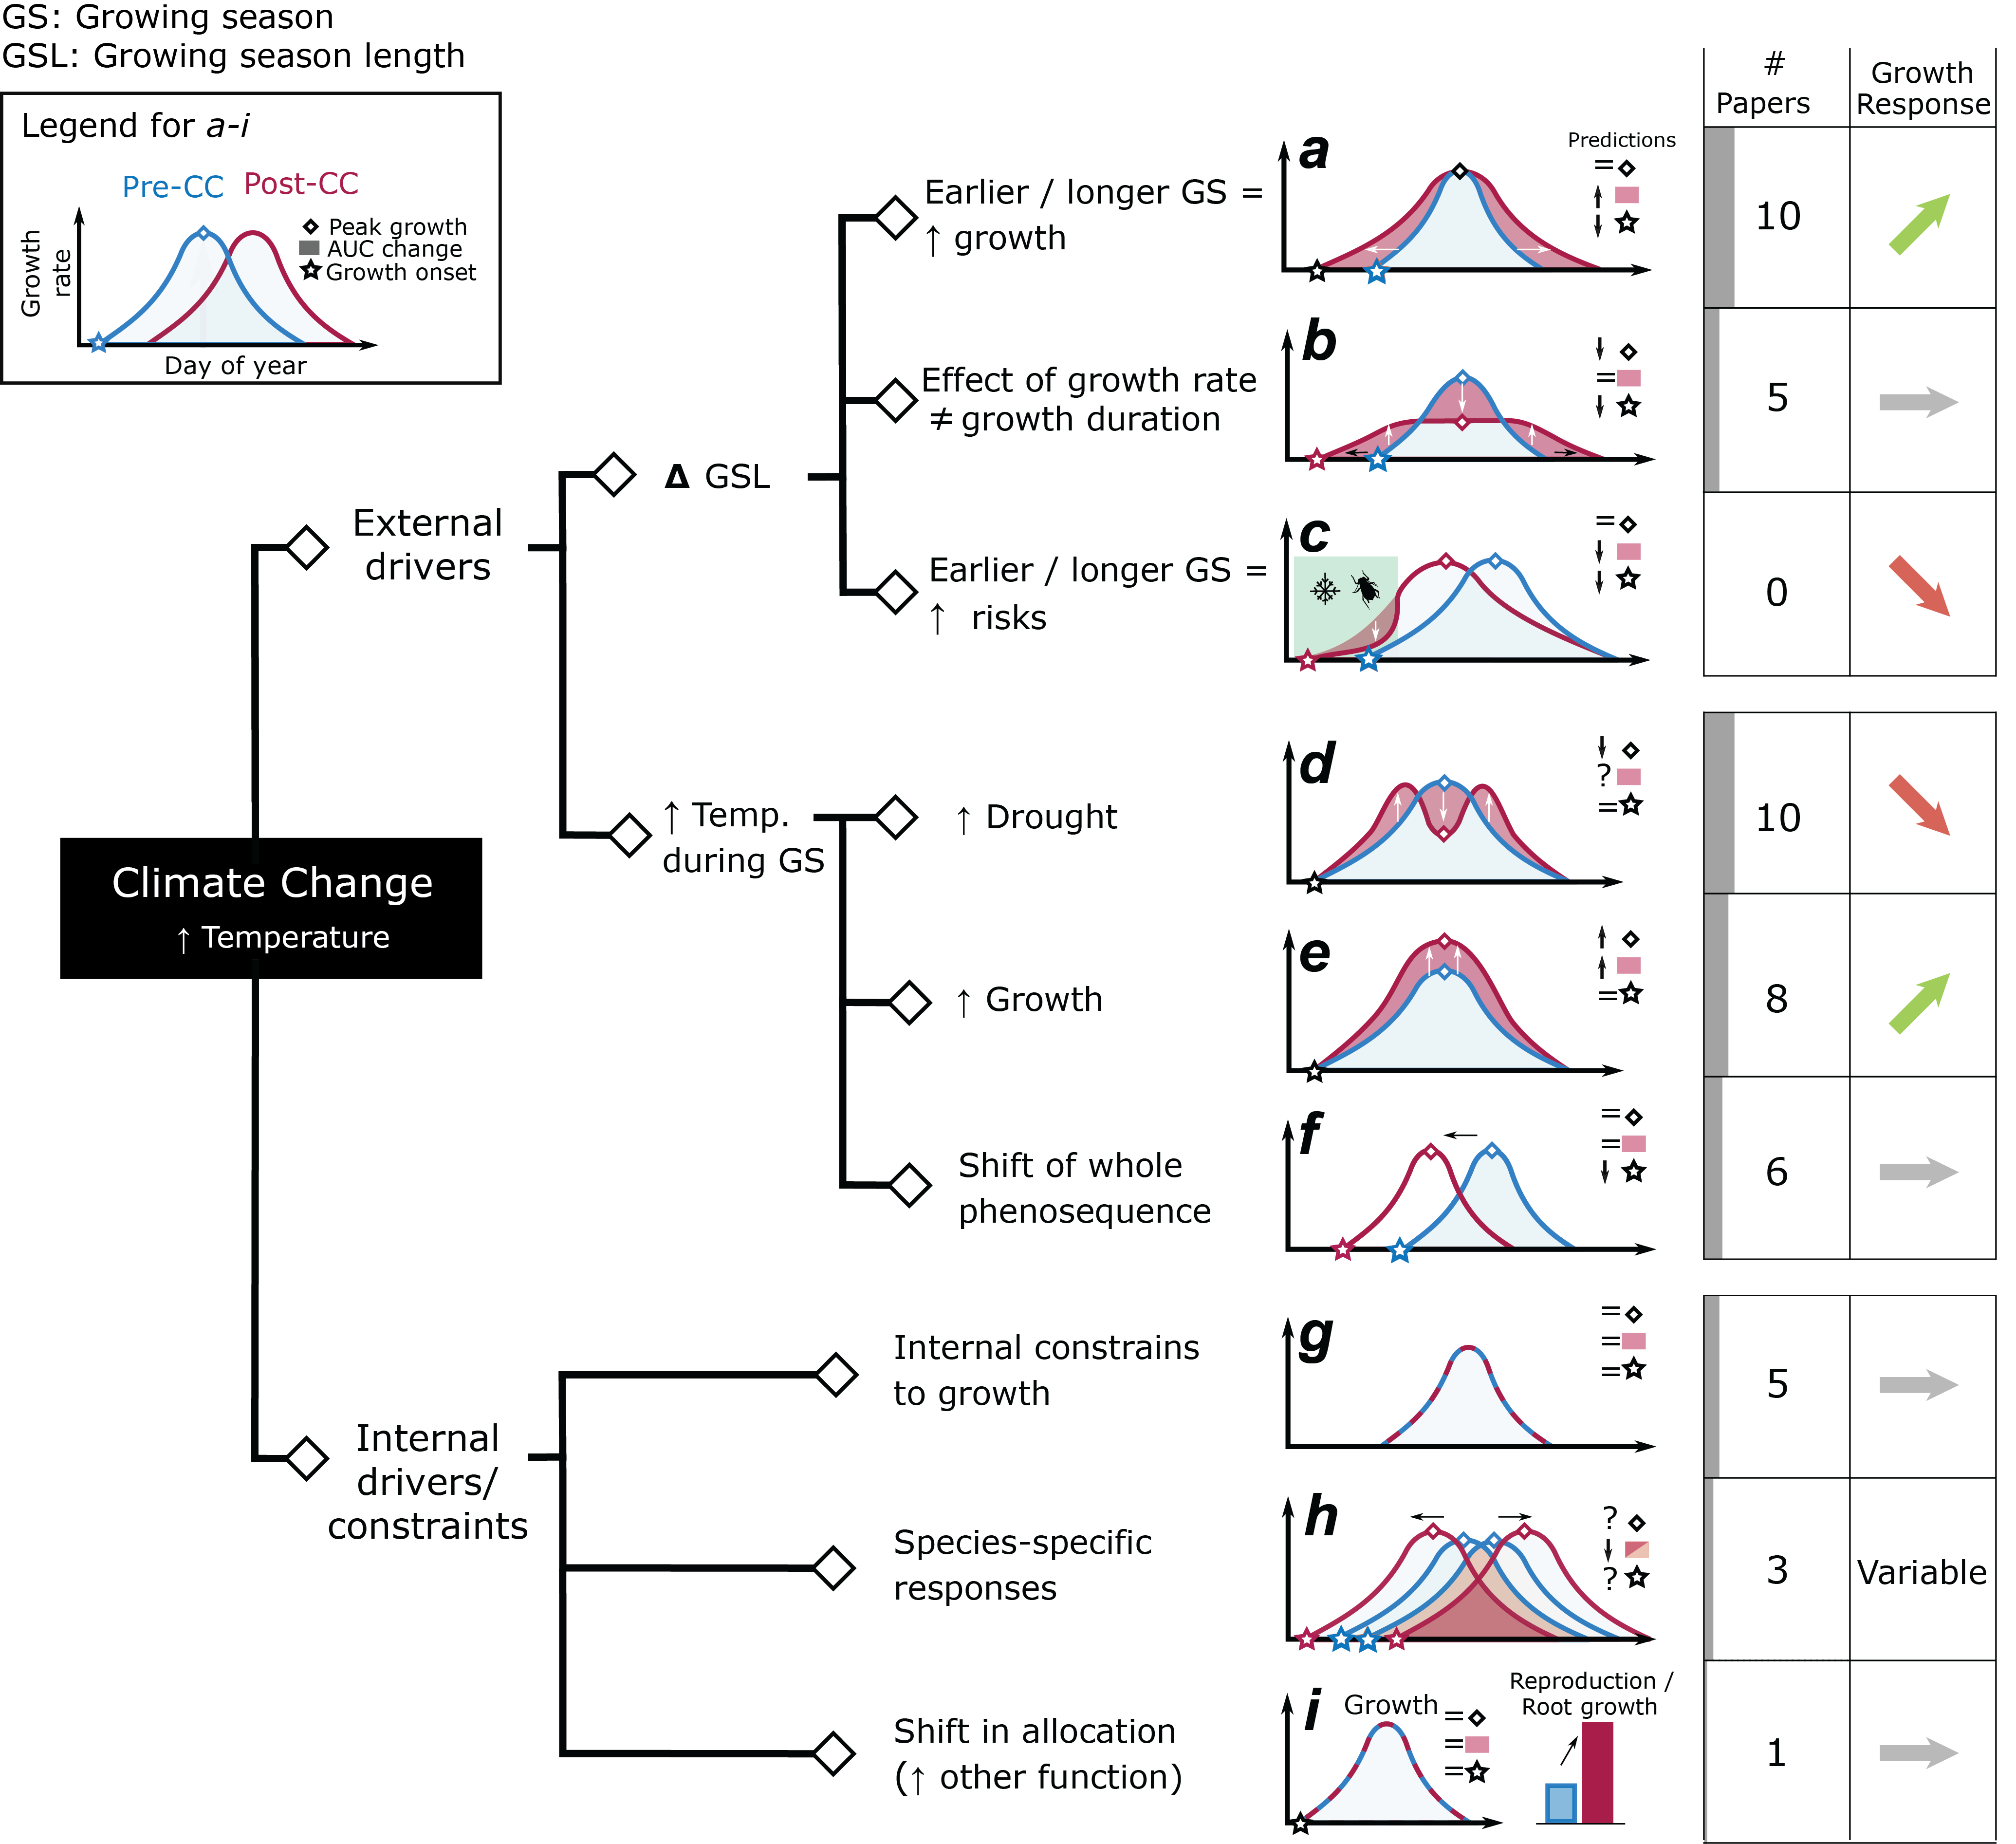
\includegraphics[width=0.9\textwidth]{..//figures/_figuresFromRuben/conceptualRev.png}
\caption{\emph{Altered growing season length (GSL) due to climate change can affect tree growth through diverse pathways.} We review hypotheses for these pathways showing the number of papers (from a review of papers studying growth $\times$ growing season length) that mentioned each hypothesis. For each graph, the peak (diamond), growth onset (start), and change in area under the curve (shading) is highlighted for the growth curves before (blue) and after (red) climate change. The right side columns highlight the number of papers studying each mechanism (left) and the expected growth response for each hypothesis (right). We group hypotheses as focused on mechanisms moderated by the environment (`external') versus those focused on internal physiological constraints, which span both source (photosynthesis-limited) and sink limitation, and could act together. For more details, see Supplement.} 
\end{figure}

\clearpage
\begin{figure}[h!]
% 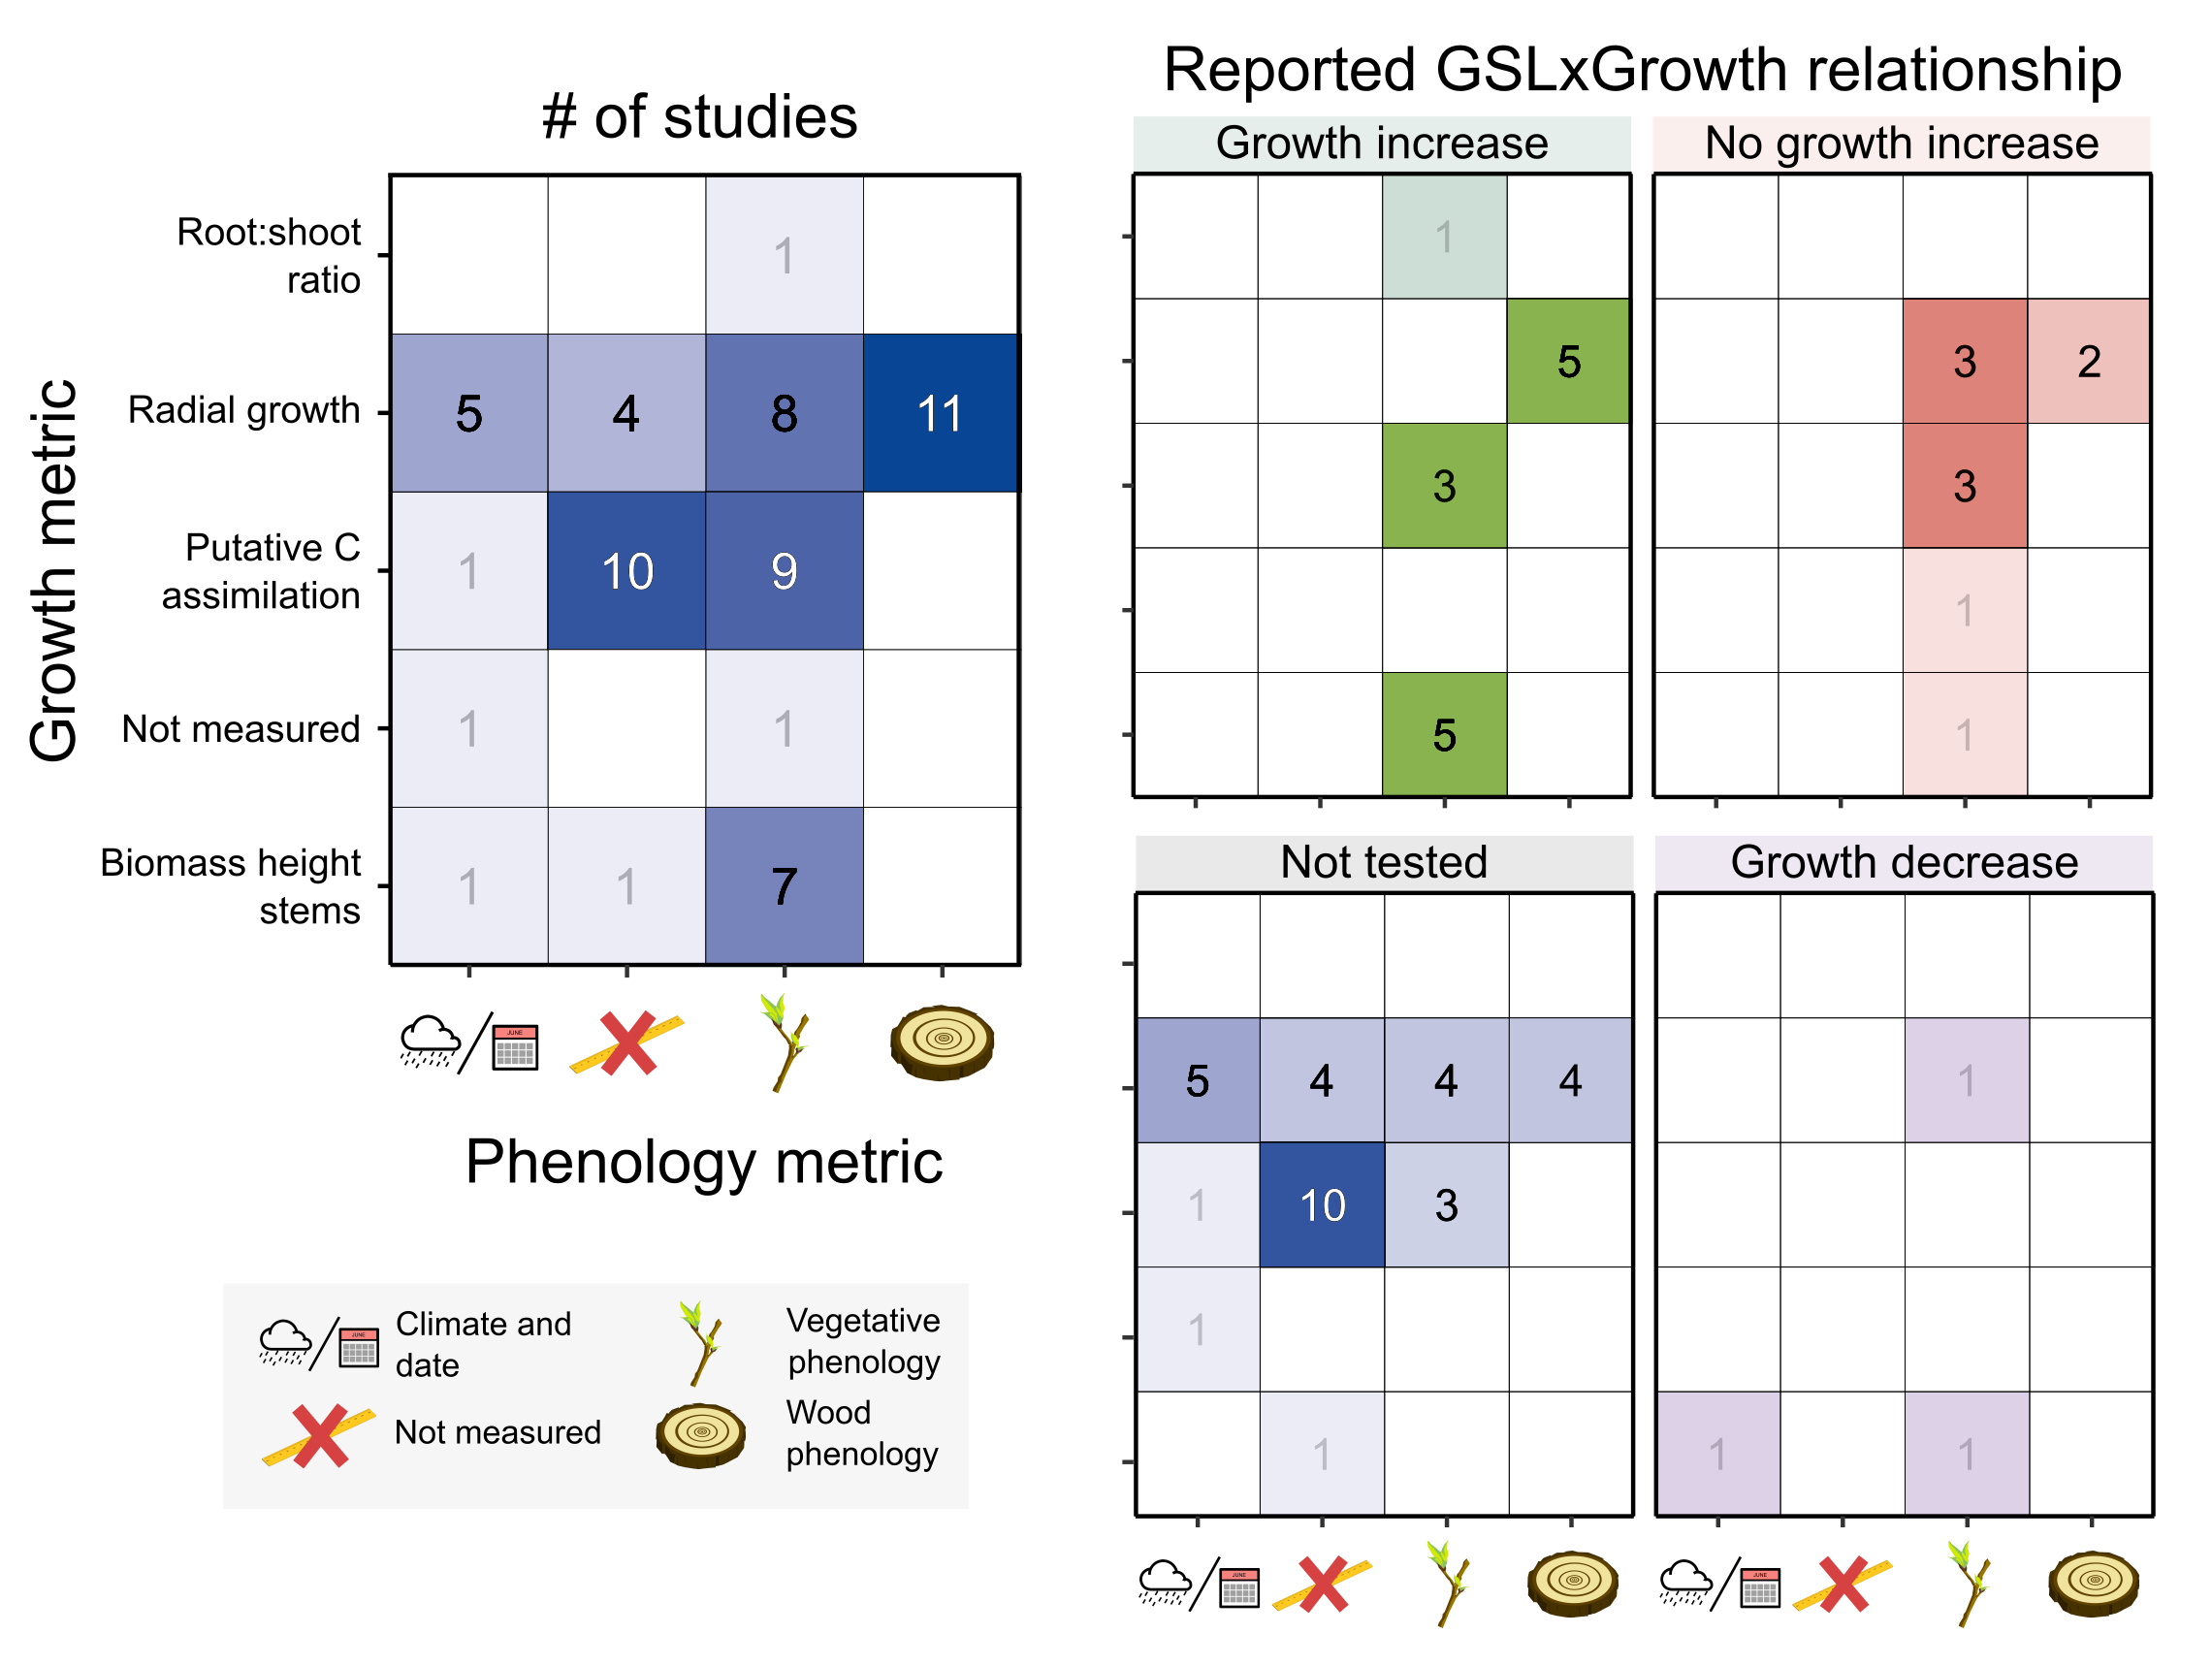
\includegraphics[width=1\textwidth]{..//figures/_figuresFromRuben/heatmap.png} 
\caption{\emph{Growth $\times$ growing season length relationships across studies and methods.} We found no coherency in which methods did or did not find a positive relationship. A number of studies tested relationships possibly related to growth $\times$ growing season length (e.g. they tested how spring temperatures related to growth) but never directly growth $\times$ growing season length, thus `not tested' was surprisingly common across methods. Left, frequency of phenological metrics and growth metrics used across the reviewed studies. Right, distribution of observed responses across these approaches. The number of papers within each combination is displayed, with shade emphasizing this value. See Supplement for review details.}
\end{figure}


\clearpage
\begin{figure}[h!]
% 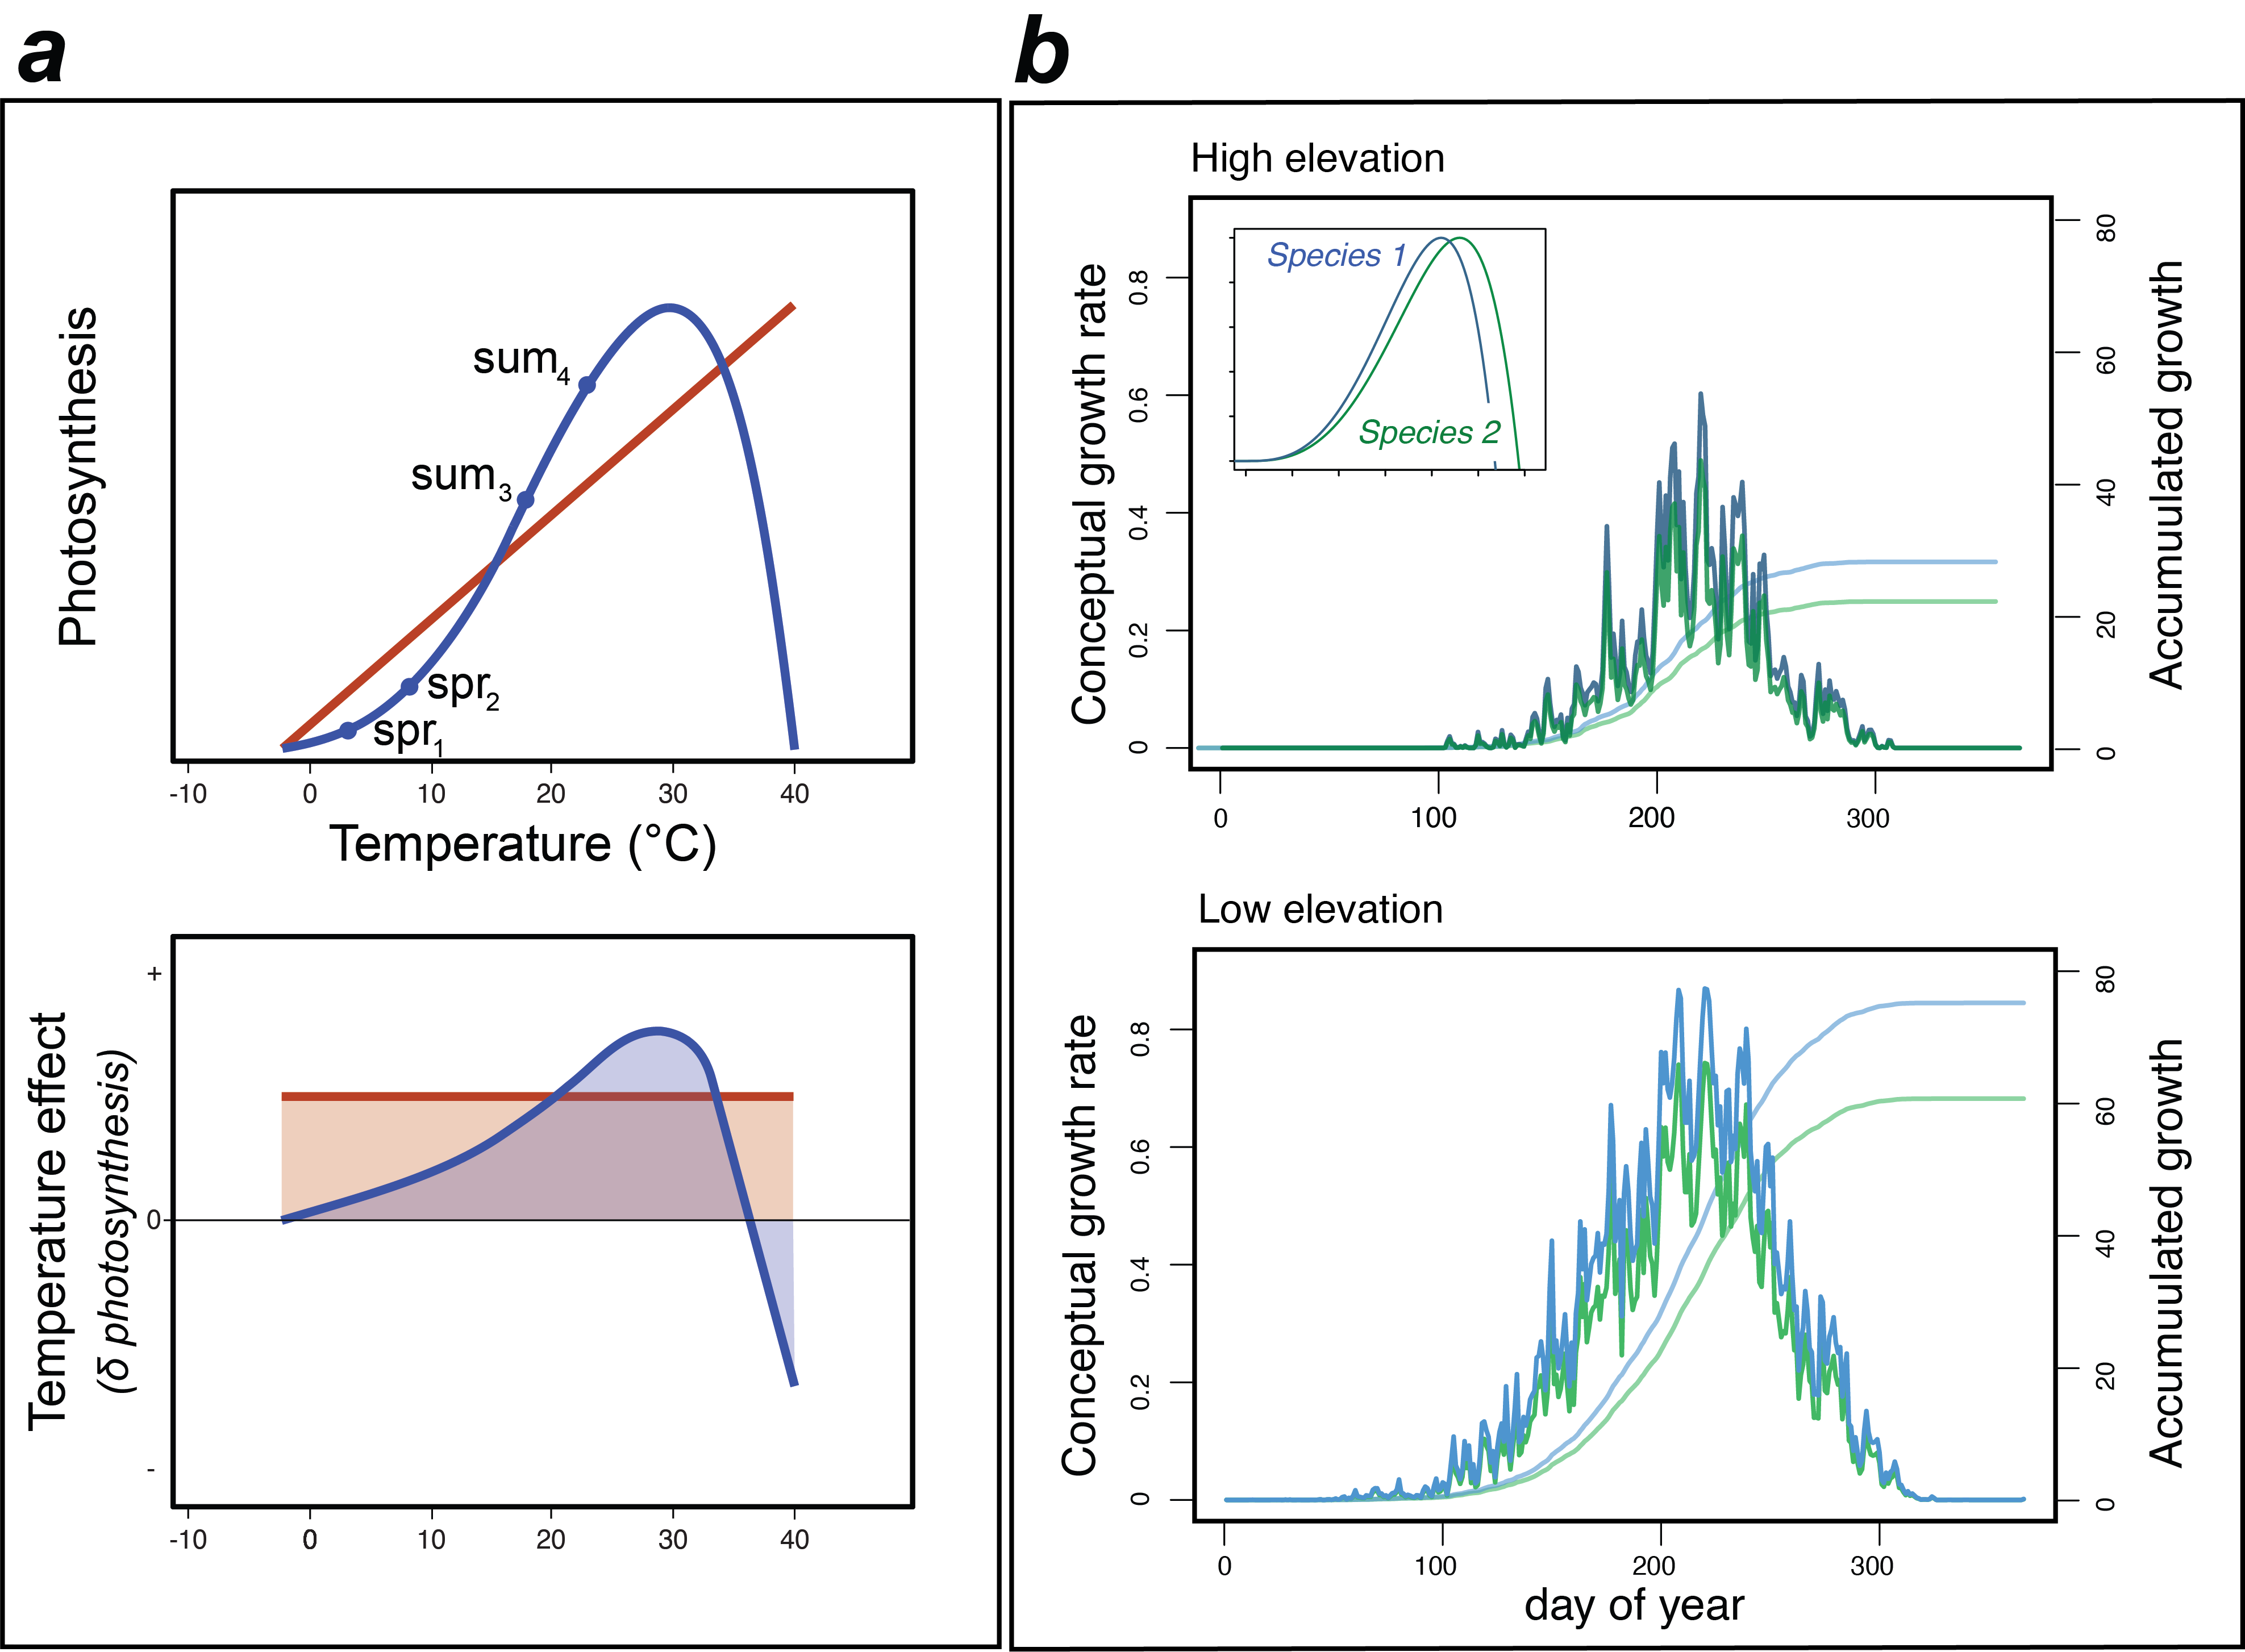
\includegraphics[width=1\textwidth]{..//figures/elevationconcept/elevationrateswtempresponse.png}
\caption{\emph{Understanding how longer seasons with climate change affect growth requires teasing out effects of longer seasons versus warmer seasons.} These two effects generally co-vary in observational data, adding complexity that we show here with two examples. a) A general net photosynthesis response curve (top panel), which has a non-linear response to temperature  \citep[blue curve, adapted from meta-analysis of][]{rezende2019thermal}, contrasts with the commonly used linear response (red). This non-linearity means that increases in lower temperatures---such as those in the spring when much of growing season extensions may happen---have lower absolute increases in photosynthesis compared to increases in later-season (e.g. summer) warmer temperatures, while a linear response assumes a constant scale of effect across low to high temperatures (bottom). b) Conceptual growth responses to temperature for two different species with different growth rate responses to temperature (top, inset), which impacts their growth across the season, leading to small absolute differences in accumulated growth at a conceptual high elevation site (top) versus larger differences in accumulated growth low elevation site (bottom). Testing how growth varies across larger spatial gradients of growing season length, as we conceptualize here (b) could help establish a baseline expectation of the scale of temporal---especially inter-annual variation---and force a greater reckoning with drivers that shift alongside growing season length.}
\end{figure}

\clearpage
\begin{figure}[h!]
% 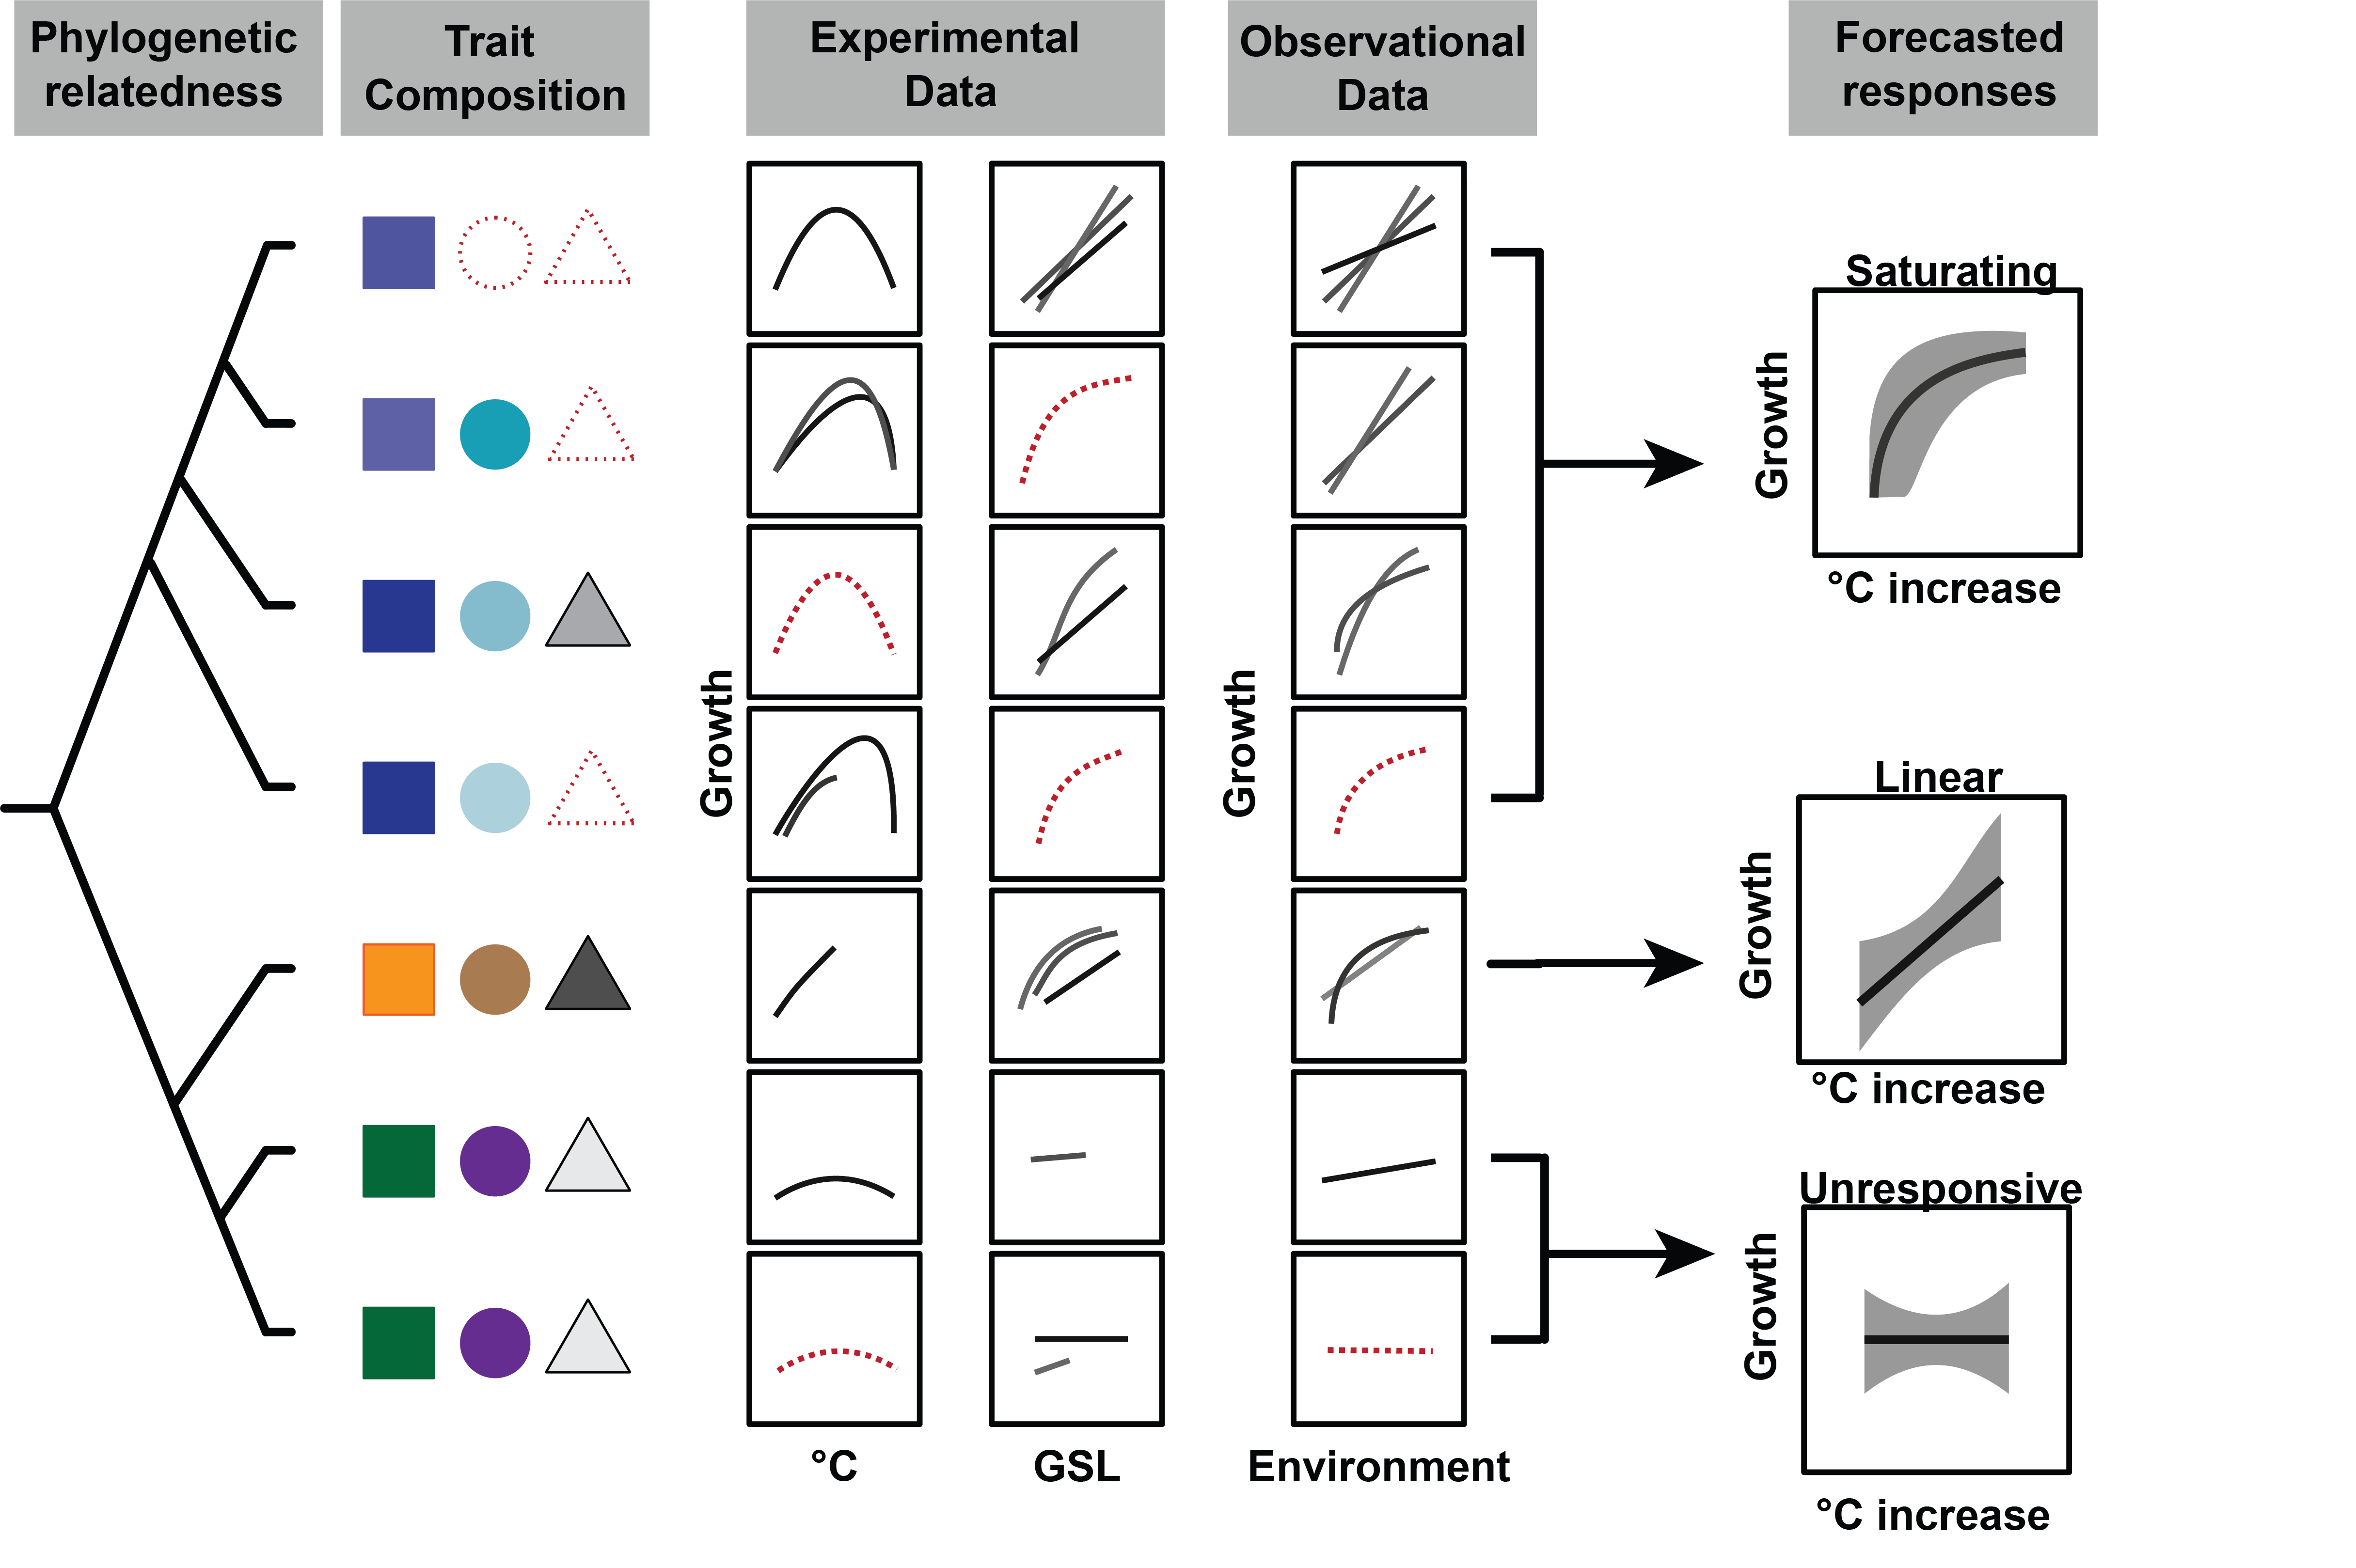
\includegraphics[width=1\textwidth]{..//figures/phylomodel/phylomodel.png}
\caption{\emph{A trait-based phylogenetic model can organize species responses to predict how they respond to longer seasons.} This approach estimates a universal model that is then shaped by species evolutionary history (shown at left via a phylogenetic tree) and traits to produce the divergent responses observed across species (and, not shown, populations) today. We argue this framework can organize and guide experiments that separate out changes in temperature from changes in growing season length (\degree C and GSL in see middle panels) to better integrate observational data and identify different responses by species that can help forecast (see `Building a new framework for growth $\times$ season length' section for more details). It also can be useful for global forecasts. For example, species-level estimates combined with data on species abundance across forests \citep[e.g.][]{FIA,fischer2019swiss} could predict larger-scale metrics, such as satellite observations of phenology and productivity. Here, this approach can identify one clade (top) with a common response to longer seasons that also shares a suite of similar traits, and can identify a unique response by one species in a clade where that species also has a unique trait compared to other species with the same common ancestor (lower clade), while handling uneven sampling and missing data (the dashed red lines represent that the model will predict a response for each species). }  
\end{figure}


\end{document}
